%
% chapter.tex
%
% (c) 2020 Prof Dr Andreas Müller
%
\chapter{Interpolation\label{chapter:interpolation}}
\lhead{Interpolation}
\rhead{}
Der Satz von Stone-Weierstrass garantiert, dass jede stetige Funktione
auf einem Interval beliebig genau durch Polynome approximiert werden
kann.
Polynome sind effizient berechenbar, es ist daher naheliegend,
komplizierte Funktione durch Polynome zu approximieren, die möglichst
viele für die vorliegende Anwendung relevante Eigenschaften mit der
Funktion gemeinsam habe.

Leider sagt der Satz von Stone-Weierstrass nichts darüber, wie solche
Polynome gefunden werden könnten.
Ziel dieses Kapitels ist daher, einige Möglichkeiten zusammenzustellen,
solche Approximationspolynome zu finden und insbesondere auch ihre
Fehler abzuschätzen.

%
% polygon.tex
%
% (c) 2020 Prof Dr Andreas Müller, Hochschule Rapperswil
%
\section{Lineare Interpolation und Polygonzüge
\label{buch:section:lineareinterpolation}}
Oft sind von einer Funktion nur einzelne Werte bekannt, doch meist reicht
dies, den ungefähren Verlauf ihres Graphen zu erahnen.
Unter der Annahme, dass sich die Funktion zwischen den bekannten Werten
nicht zu ``wild'' verhält, können Werte zwischen den bekannten Werten
abgeschätzt werden.
In diesem Abschnitt soll daher die folgende Aufgabe gelöst werden.

\begin{aufgabe}
\label{buch:aufgabe:basicinterpolation}
Gegeben $n+1$ sogenannte {\em Stützstellen}
\index{Stützstelle}%
\[
a=x_0<x_1<x_2<\cdots<x_{n-1}<x_n=b
\]
im Intervall $[a,b]$ und bekannte Funktionswerte $f_i$, $0\le i\le n$,
finde eine stetige Funktion $f\colon[a,b]\to \mathbb R$ derart, dass
$f(x_j)=f_j$ für $0\le j\le n$.
\end{aufgabe}

\subsection{Lineare Interpolation
\label{buch:subsection:lineareinterpolation}}
Die Aufgabe~\eqref{buch:aufgabe:basicinterpolation} ist zu wenig präzise
gestellt, es gibt unendlich viele Lösungen.
\index{lineare!Interpolation}%
\index{Interpolation!linear}%
Es müssen daher zusätzliche Bedingungen an die gesuchte Funktion $f$
gestellt werden, damit die Lösung eindeutig bestimmt wird.
Ein mögliche solche Bedingung ist, dass die Funktion $f$ in jedem
Teilintervall zwischen aufeinanderfolgenden Stützstellen linear ist.
In diesem Fall haben die Werte ausserhalb des Intervalls offenbar 
keinen Einfluss auf den Verlauf im Inneren des Intervalls, es genügt
also das Problem mit nur zwei Stützstellen zu lösen.

\begin{satz}
\label{buch:satz:lineareinterpolation}
Die einzige auf dem Intervall $[x_i,x_{i+1}]$ definierte lineare Funktion 
\index{lineare!Funktion}%
\index{Funktion!linear}%
$f(x)$ mit Funktionswerten $f(x_i)=f_i$ und $f(x_{i+1}) = f_{i+1}$
hat im Punkt $x\in[x_i,x_{i+1}]$
den Wert
\begin{equation}
f(x)
=
\frac{f_{i+1}-f_i}{x_{i+1}-x_i} (x-x_i) + f_i
=
\frac{x-x_{i+1}}{x_i-x_{i+1}} f_i
+
\frac{x_{i}-x}{x_i-x_{i+1}} f_{i+1}
=
f_il_i(x) + f_{i+1}l_{i+1}(x)
\label{buch:eqn:lineareinterpolation}
\end{equation}
mit den linearen Funktionen
\begin{equation}
l_i(x) = \frac{x-x_{i+1}}{x_i-x_{i+1}}
\qquad\text{und}\qquad
l_{i+1}(x) = \frac{x_i-x}{x_i-x_{i+1}}.
\label{buch:eqn:linl0l1}
\end{equation}
\end{satz}

\begin{proof}[Beweis von Satz~\ref{buch:satz:lineareinterpolation}]
Die beiden linearen Funktion $l_i(x)$ und $l_{i+1}(x)$ haben an den 
Intervallenden die speziellen Werte
\[
\begin{aligned}
l_i(x_i)&=1  &\qquad&\qquad& l_{i+1}(x_i)&=0 \\
l_i(x_i)&=0  &\qquad&\qquad& l_{i+1}(x_i)&=1,
\end{aligned}
\]
wie man durch Einsetzen unmittelbar bestätigen kann.
Die zweite Form in~\eqref{buch:eqn:lineareinterpolation}
ist daher als Linearkombination
\[
f(x)=f_il_i(x) + f_{i+1}l_{i+1}(x)
\]
linearer Funktionen wieder
linear und dank der speziellen Werte von $l_i$ und $l_{i+1}$ folgt
unmittelbar, dass
\begin{align*}
f(x_i)&=f_il_i(x_i) + f_{i+1}l_{i+1}(x_i) = f_i\cdot 1 + f_{i+1}\cdot 0= f_i\\
f(x_{i+1})&=f_il_i(x_{i+1}) + f_{i+1}l_{i+1}(x_{i+1})= f_i\cdot 0 + f_{i+1}\cdot 1=f_{i+1}
\end{align*}
gilt.

Der Bruch
\index{Bruch}%
\[
m = \frac{f_{i+1}-f_i}{x_{i+1}-x_i}
\]
ist die Steigung der Geraden durch die Punkte $(x_i,f_i)$ und
$x_{i+1},f_{i+1})$.
\index{Steigung}%
Der erste Ausdruck auf der rechten Seite in
\eqref{buch:eqn:lineareinterpolation} ist
also $f(x)=m(x-x_i)+f_i$, dies ist die Gleichung einer Geraden
mit Steigung $m$ durch den Punkt $(x_i,f_i)$, sie verläuft natürlich
auch durch den Punkt $(x_{i+1},f_{i+1})$.
\index{Gerade}%
\end{proof}


\subsection{Polygonzüge
\label{buch:subsection:polygonzuege}}
\begin{figure}
\centering
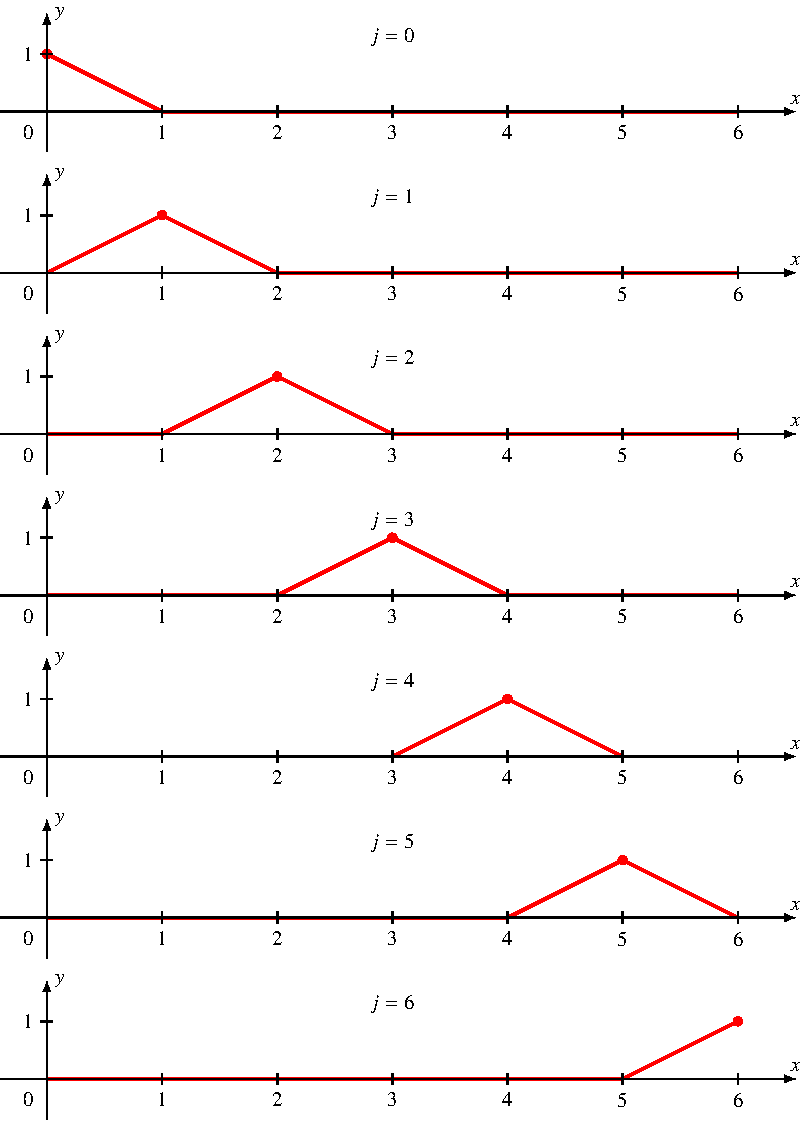
\includegraphics{chapters/30-interpolation/figures/polygon.pdf}
\caption{Basisfunktionen für die lineare Interpolation einer 
Funktion $f\colon[0,6]\to\mathbb R$ mit Stützstellen $0,1,\dots,6$
\label{buch:figure:polygonbasis}}
\end{figure}
\eqref{buch:eqn:linl0l1}
Wendet man das Resultate von Satz~\ref{buch:satz:lineareinterpolation}
auf jedes Teilintervall an, entsteht eine Interpolationsfunktion, deren
Graph ein Polygonzug ist.
\index{Interpolationsfunktion}%
\index{Graph}%
\index{Polygonzug}%
Eine solche Funktion lässt sich einfacher beschreiben mit Hilfe
der Interpolationsfunktionen mit den speziellen Werten
\begin{equation}
l_i(x_j) = \delta_{ij} =\begin{cases}
1&\qquad i=j\\
0&\qquad\text{sonst.}
\end{cases}
\label{buch:eqn:interpolation:basis}
\end{equation}
Die Funktionen sind in Abbildung~\ref{buch:figure:polygonbasis} für
die Stütztstellen $x_0=0$, $x_1=1$, \dots , $x_6=6$ dargestellt.
Die lineare Interpolationsfunktion kann jetzt als Linearkombination
der Funktionen $l_i$ geschrieben werden:
\begin{equation}
f(x)
=
\sum_{j=0}^n f_j l_j(x).
\label{buch:eqn:interpolation:linearkombination}
\end{equation}
Diese Lösung des Interpolationsproblems kann für alle weiteren
Interpolationsansätze in diesem Kapitel als Vorlage dienen.
Es geht nämlich nicht darum, eine Interpolationsfunktion in
geschlossener Form hinzuschreiben, dies ist für die Funktionen $l_j(x)$
ohnehin nicht möglich.
Es ist nur nötig, dass Funktionswerte $f(x)$ effizient berechnet
werden können.
Die letztere Aufgabe ist gelöst, wenn man die Funktionen $l_j(x)$
effizient berechnen kann.
Es ist dann nur noch die
Linearkombination~\eqref{buch:eqn:interpolation:linearkombination}
zu bilden.

Die Wahl der Funktionen $l_j(x)$, die natürlich die Bedingungen
\eqref{buch:eqn:interpolation:basis} erfüllen müssen,
bestimmt die Eigenschaften der
Interpolationsfunktion, die nach 
\eqref{buch:eqn:interpolation:linearkombination}
gebildet wird.
In diesem Abschnitt waren die $l_j$ stückweise lineare Funktionen,
also auch die Funktion $f(x)$.
\index{stückweise linear}%
Im nächsten Abschnitt sollen die Funktionen Polynome sein,
also wird die Interpolationsfunktion ebenfalls ein Polynom sein.







%
% polynom.tex
%
% (c) 2020 Prof Dr Andreas Müller, Hochschule Rapeprswil
%
\section{Interpolationspolynom
\label{buch:section:interpolationspolynom}}
\rhead{Lagrange-Interpolationspolynome}
In diesem Abschnitt wird die folgende Aufgabe gelöst.
\begin{aufgabe}[Interpolationspolynom]
\index{Interpolationspolynom}%
Gegeben Stützstellen
\[
a=x_0<x_1<x_2<\dots < x_{n-1}<x_n=b
\]
und Funktionswerte $f_i, 0\le i\le n$, finde ein Polynom $l(x)$
mit der Eigenschaft $l(x_i)=f_i$ für alle $i=0,1,\dots n$.
\end{aufgabe}
Gegeben sind also $n+1$ Bedingungen, die das Polynom erfüllen muss.
Abgesehen von trivialen Fällen wie dem Null-Polynom, muss ein Polynom
im Allgemeinen mindestens den Grad $n$ haben, damit alle 
Bedingungen durch geeignete Wahl der $n+1$ Koeffizienten erfüllt werden können.
\index{Nullpolynom}%
Man könnte das Polynom nämlich in der Form
\[
p(x)
=
a_nx^n + a_{n-1}x^{n-1}+\dots+a_1x+a_0
\]
ansetzen und die Stützstellen einsetzen.
\index{Stützstellen}%
Lösung des Gleichungssystem
\index{Gleichungssystem!für das Interpolationspolynom}%
\begin{equation}
\begin{linsys}{5}
{\color{red}a_N}x_0^N &+& {\color{red}a_{N-1}}x_0^{N-1} &+& \dots &+& {\color{red}a_1}x_0 &+& {\color{red}a_0}x_0 &=& f_0 \\[5pt]
{\color{red}a_N}x_1^N &+& {\color{red}a_{N-1}}x_1^{N-1} &+& \dots &+& {\color{red}a_1}x_1 &+& {\color{red}a_0}x_1 &=& f_1 \\[5pt]
\vdots   & &    \vdots        & & \ddots& & \vdots & & \vdots & & \vdots\\[5pt]
{\color{red}a_N}x_n^N &+& {\color{red}a_{N-1}}x_n^{N-1} &+& \dots &+& {\color{red}a_1}x_n &+& {\color{red}a_0}x_n &=& f_n 
\end{linsys}
\end{equation}
für die Koeffizienten $\color{red}a_k$
liefert dann die gesuchten Koeffizienten.
\index{Koeffizient}%
Dieser Weg ist allerdings sehr aufwendig, die Lösung eines linearen
Gleichungssystems mit dem Gauss-Algorithmus benötigt $O(n^3)$ Operationen.
\index{Gauss-Algorithmus}%
Die sehr spezielle Struktur des Gleichungssystems sollte ermöglichen,
das Polynom $l(x)$ auf direkterem Weg zu ermitteln.

%
% Interpolationspolynom bestimmen
%
\subsection{Bestimmung des Interpolationspolynoms
\label{buch:section:interpolation:bestimmung}}
Das allgemeine Interpolationsproblem kann leicht gelöst werden, wenn
das folgende spezielle Interpolationsproblem gelöst ist.
\index{Interpolationspolynom!spezielles}%
\index{spezielles Interpolationspolynom}%

\begin{aufgabe}[Spezielle Interpolationspolynome]
\label{buch:aufgabe:speziellesinterpolationsproblem}
Gegeben die Stützstellen
\[
a=x_0<x_1<x_2<\dots <x_{n-1}<x_n=b,
\]
finde Polynome $l_j$ vom Grad $n$ derart, dass
\[
l_j(x_i) = \delta_{ij}=\begin{cases}
1&\qquad i=j\\
0&\qquad\text{sonst.}
\end{cases}
\]
\end{aufgabe}

\begin{figure}
\centering
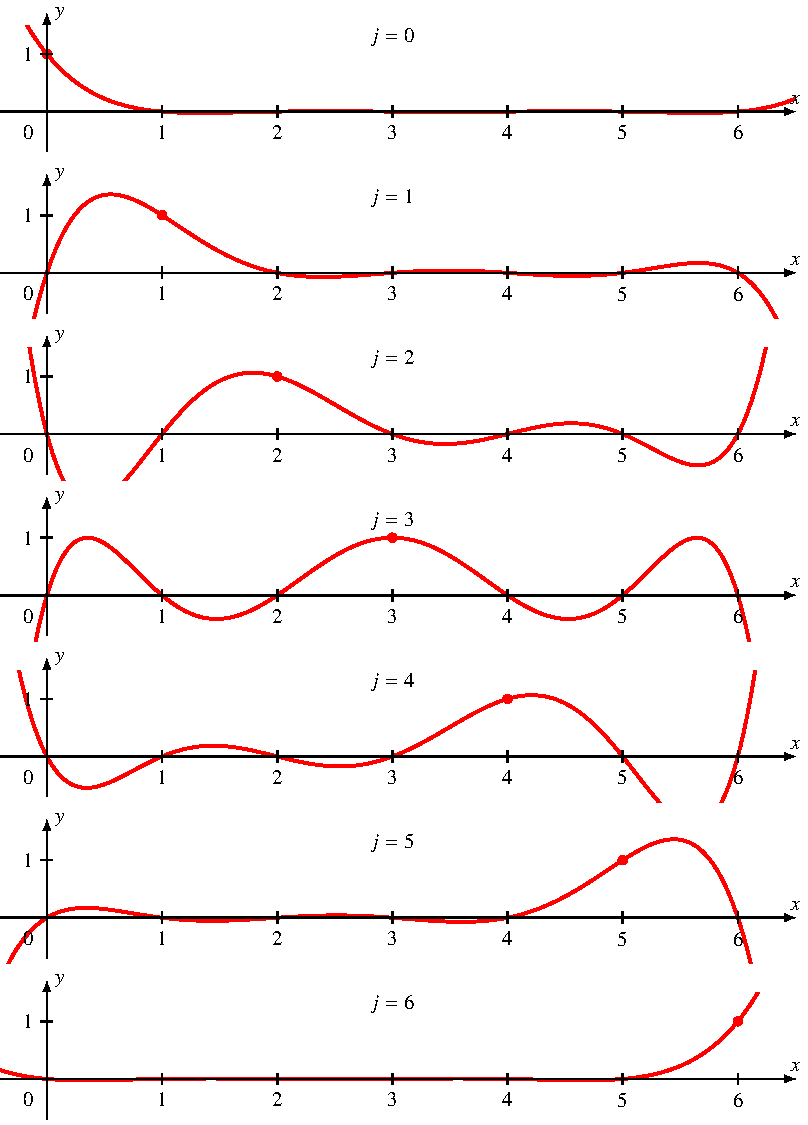
\includegraphics{chapters/30-interpolation/figures/basis.pdf}
\caption{Polynome $l_j(x)$, welche des spezielle Interpolationsproblem
\ref{buch:aufgabe:speziellesinterpolationsproblem}
lösen.
\label{buch:figure:spezielleinterpolation}}
\end{figure}

Jedes der Interpolationspolynome $l_j$ hat Grad $n$, also hat auch eine
beliebige Linearkombination den Grad höchstens $n$.
\index{Linearkombination}%
Die Linearkombination
\[
p(x) = \sum_{j=0}^n f_j l_j(x)
\]
ist das gesuchte Interpolationspolynom, wie Einsetzen von $x_i$ in
\[
p(x_i)
=
\sum_{j=0}^n f_jl_j(x_i)
=
\sum_{j=0}^n f_j\delta_{ij}
=
f_i
\]
bestätigt.

\begin{beispiel}
Ein besonders einfacher Fall ist $n=1$.
Gesucht ist eine lineare Funktion $l(x)=a_1x+a_0$ derart, dass
$l(x_0)=f_0$ und $l(x_1)=f_1$.
Polynome $l_0$ und $l_1$ können leicht angegeben werden:
\[
l_0(x) = \frac{x_1-x}{x_1-x_0}
\qquad\text{und}\qquad
l_1(x) = \frac{x-x_0}{x_1-x_0}
\]
haben die geforderten Eigenschaften.
Die gesuchte Interpolationsfunktion ist daher
\[
p(x)
=
\frac{x_1-x}{x_1-x_0}f_0 + \frac{x-x_0}{x_1-x_0} f_1
=
x \frac{f_1-f_0}{x_1-x_0}   + \frac{x_1f_0-x_0f_1}{x_1-x_0}.
\]
Der Koeffizient von $x$ ist wie erwartet die Steigung der Geraden durch
die Punkte $(x_0,f_0)$ und $(x_1,f_1)$.
\end{beispiel}

Ein Polynom vom Grad $n+1$, welches in {\em allen} Stützstellen verschwindet,
ist leicht zu finden, es ist 
\[
l(x)
=
(x-x_0)(x-x_1)(x-x_2)\cdots (x-x_{n-1})(x-x_n).
\]
\index{lx@$l(x)$}%
Ein Polynom, welches nur an der Stützstelle $x_j$ {\em nicht} verschwindet,
ensteht, indem man den Faktor $(x-x_j)$ weglässt, es hat den Grad $n$.
Wir führen dafür die Notation
\[
(x-x_0)(x-x_1)(x-x_2)\cdots \widehat{(x-x_j)}\cdots (x-x_{n-1})(x-x_n),
\]
der Hut bedeutet, dass dieser Faktor weggelassen werden soll.
Allerdings hat dieses Polynom nicht den geforderten Wert $1$, man muss es
also noch mit einer geeigneten Konstante multiplizieren.
Das gesuchte Polynom $l_j(x)$ hat daher die Form
\[
l_j(x)
=
c_j(x-x_0)(x-x_1)(x-x_2)\cdots \widehat{(x-x_j)}\cdots (x-x_{n-1}(x-x_n).
\]
Einsetzen von $x_j$ ergibt
\[
l_j(x_j) = 1 = 
c_j(x_j-x_0)(x_j-x_1)(x_j-x_2)\cdots \widehat{(x_j-x_j)}\cdots(x_j-x_{n-1})(x_j-x_n),
\]
\index{ljx@$l_j(x)$}%
die Konstante $c_j$ ist daher
\[
c_j = \prod_{i=0\atop i\ne j}^n \frac{1}{x_j-x_i}.
\]

\begin{beispiel}
Man finde ein Polynome, welches $l(0)=l(1)=0$ und $l(\frac12)=1$
erfüllt.
Wegen $f_0=f_2=0$ ist nur das Polynom $l_1$ zu ermitteln, es ist
\[
l(x) = l_1(x)
=
\frac{(x-x_0)(x-x_2)}{(x_1-x_0)(x_1-x_2)}
=
\frac{x(x-1)}{\frac12(\frac12-1)}
=
\frac14x(1-x).
\qedhere
\]
\end{beispiel}

%
% Fehler des Interpolationspolynoms
%
\subsection{Fehler von Approximationspolynomen
\label{buch:section:interpolation:fehler}}
Getreu der Maxime, dass wir zu jeder numerischen Lösungsformel auch
Informationen über die zu erwartenden Fehler brauchen, entwickeln
wir in diesem Abschnitt die Theorie des Fehlers der Approximationspolynome.
\index{Fehler des Approximationspolynoms}%
Wir müssen zu diesem Zweck einen kleinen Ausflug in die Analysis unternehmen
in einen Bereich, der im Unterricht manchmal etwas zu kurz kommt.

Wenn die Ableitung einer Funktion in einem Intervall klein ist,
dann werden auch die Funktionswerte im Inneren dieses Intervalls
nicht gross von den Werten am Rand abweichen können.
Eine grosse Abweichung würde ja automatisch eine Steigung einer Sekanten
und damit auch eine grosse Steigung einer Tangenten zur Folge haben.
\index{Sekante}%
\index{Tangente}%
Dies ist die Idee, die den nachfolgend entwickelten Fehlerabschätzungen
zu Grunde liegt.
\index{Fehlerabschätzung}%

\subsubsection{Der Zwischenwertsatz}
\index{Zwischenwertsatz}%
Der Ausgangspunkt aller nachfolgenden Überlegungen ist die intuitiv
anschauliche Tatsache, dass eine stetige Funktion keine Sprünge macht.

\begin{satz}[Zwischenwertsatz]
Eine auf dem Intervall $[a,b]$ stetige Funktion nimmt jeden Wert im
Intervall $[f(a),f(b)]$ an.
Anders ausgedrückt, für jedes $y$ zwischen $f(a)$ und $f(b)$ gibt es ein 
$x$ zwischen $a$ und $b$ derart, dass $y=f(x)$.
\end{satz}

Dieser Satz war natürlich bereits die Grundlage des Verfahrens der
Intervallhalbierung, mit welchem wir in
Abschnitt~\ref{buch:subsection:intervallhalbierung}
Gleichungen gelöst haben.
\index{Intervallhalbierung}%
Wenn die Funktion an den Intervallenden verschiedene Vorzeichen hat,
dann muss es eine Nullstelle im Inneren des Intervalls geben.
\index{Nullstelle}%
Die Intervallhalbierung hat in jedem Schritt ein neues Intervall
konstruiert, das die Nullstelle enthielt.

\subsubsection{Der Satz von Rolle}
\begin{figure}
\centering
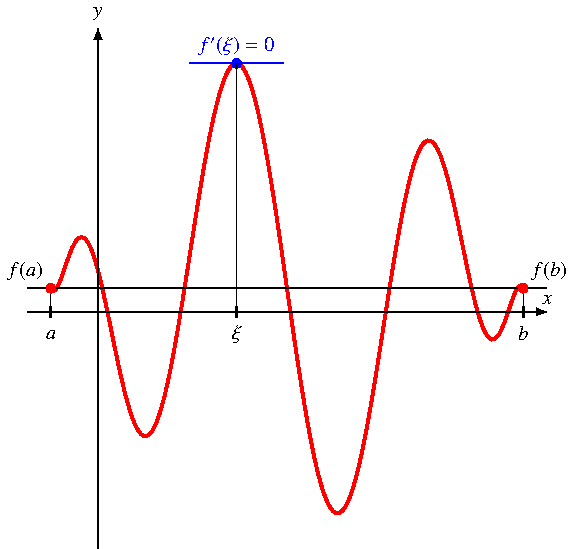
\includegraphics{chapters/30-interpolation/figures/rolle.pdf}
\caption{Satz von Rolle: eine nicht konstante differenzierbare Funktion,
die an den Enden eines Intervalls den gleichen Funktionswert hat, hat im 
Inneren des Intervalls eine Stelle $\xi$ mit Ableitung $0$.
\label{buch:figure:rolle}}
\end{figure}
Der Satz von Rolle erweitert den Zwischenwertsatz auf die Ableitung einer
differenzierbaren Funktion an (Abbildung~\ref{buch:figure:rolle}).

\begin{satz}[Rolle]
\label{buch:satz:rolle}
\index{Satz von Rolle}%
\index{Rolle, Satz von}%
Sei $f$ eine auf dem Intervall $[a,b]$ nicht konstante,
stetig differenzierbare Funktion
mit $f(a)=f(b)$, dann gibt es einen Punkt $\xi\in(a,b)]$ im Inneren
des derart, dass $f'(\xi)=0$.
\end{satz}

Der Satz von Rolle ist eine Selbstverständlichkeit, wenn die Ableitung
$f'(x)$ stetig ist, doch dies wird nicht vorausgesetzt, es wird nur
verlangt, dass die Ableitung existiert.
Ausserdem macht der Satz eine Aussage darüber, dass die Zwischenstelle
$\xi$ im Inneren des Intervalls sei.

\begin{proof}[Beweis]
Eine stetige Funktion hat auf dem kompakten Intervall $[a,b]$ mindestens
ein Maximum und ein Minimum.
Da die Funktion nicht konstant ist, ist das Maximum oder das Minimum
von $f(a)$ verschieden.
Wir nehmen an $\xi\in[a,b]$ sei ein Maximum mit dieser Eigenschaft,
das Argument für das Minimum ist völlig analog.
Wegen $f(\xi)>f(a)$ ist $\xi$ ein Punkt im Inneren des Intervalls,
also kann $\xi$ nicht $=a$ sein, folglich ist $\xi\in(a,b)$.

Wegen $f(\xi) \ge f(x)\forall x\in[a,b]$
folgt dann
\begin{align*}
f'(\xi) &= \lim_{h\to 0+}  \frac{f(\xi+h)-f(\xi)}{h} \le 0
\\
f'(\xi) &= \lim_{h\to 0-}  \frac{f(\xi+h)-f(\xi)}{h} \ge 0.
\end{align*}
Da $f$ differenzierbar ist, müssen diese beiden Grenzwerte übereinstimmen,
also ist $f'(\xi)=0$.
\end{proof}


\subsubsection{Nullstellen und der Satz von Rolle}
\begin{figure}
\centering
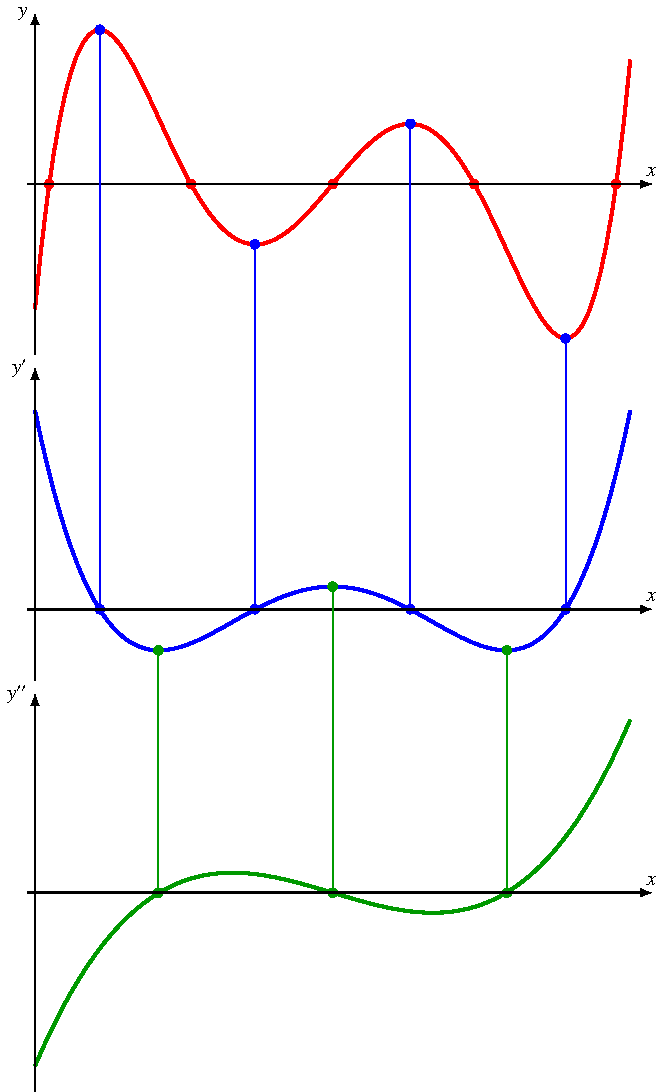
\includegraphics{chapters/30-interpolation/figures/nullstellen.pdf}
\caption{Schachtelung der Nullstellen von $f(x)$, $f'(x)$ und $f''(x)$.
Der Satz von Rolle~\ref{buch:satz:rolle} impliziert, dass sich zwischen zwei
Nullstellen von $f$ immer eine Nullstelle von $f'$ befindet, und
ebenso zwischen zwei Nullstellen von $f'$ eine von $f''$.
\label{buch:figure:nullstellen}}
\end{figure}
Ist $p(x)$ ein Interpolationspolynom für die Funktion $f(x)$, dann ist
$f(x_i)-p(x_i)=0$ für alle Stützstellen.
Insbesondere macht der Satz von Rolle Aussagen über 
die Differenz $f(x)-p(x)$ zwischen den Stützstellen.
Diese Frage wird im folgenden Satz genauer untersucht.

\begin{satz}
\label{buch:satz:nullstellen}
Ist $f$ eine differenzierbare Funktion auf dem Intervall $[a,b]$
mit Nullstellen 
\[
a=x_0 < x_1 < x_2 < \dots < x_{n-1} < x_n = b,
\]
die auf keinem Teilintervall $[x_i,x_{i+1}]$ konstant ist,
dann hat $f'$ im Inneren jedes Teilintervalls $[x_i, x_{i+1}]$
eine Nullstelle.
\end{satz}

Das Polynom 
\[
l(x) = (x-x_0)(x-x_1)\dots (x-x_{n-1})(x-x_n),
\]
welches für die Konstruktion des Interpolationspolynoms verwendet
wurde, hat genau die Nullstellen $x_0,x_1,\dots,x_{n-1},x_n$.
Nach dem Satz~\ref{buch:satz:nullstellen} muss es zwischen je
zwei aufeinanderfolgenden Nullstellen von $l$ eine Nullstelle der
Ableitung geben. 
Diese Situation ist in Abbildung~\ref{buch:figure:nullstellen}
für den Fall $l(x)=(x+2)(x+1)x(x-1)(x-2)$ dargestellt.

Die höheren Ableitungen $f^{(k)}$ haben ihre Nullstellen
natürlich auch wieder zwischen den Nullstellen der Ableitung $f^{(k-1)}$.
Die $n$-te Ableitung ist konstant und hat keine Nullstellen.

%\begin{figure}
%\centering
%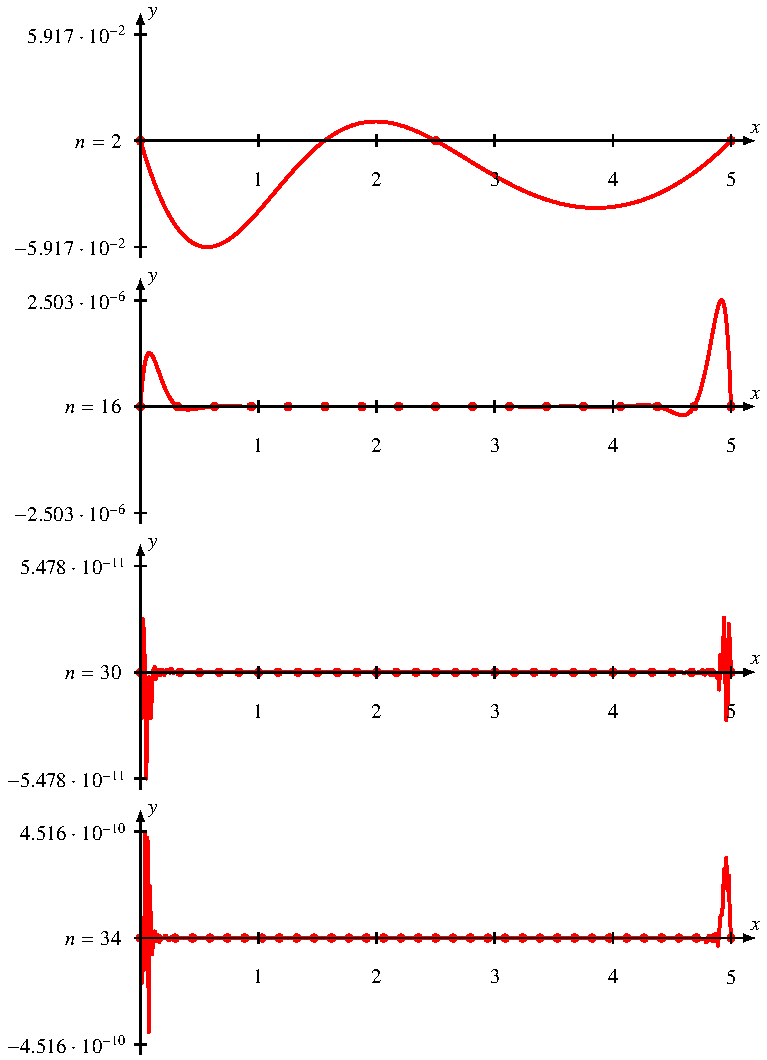
\includegraphics{chapters/30-interpolation/figures/norm.pdf}
%\caption{Fehler des Lagrange-Interpolationspolynoms für die Funktion
%$f(x)=e^{-x^2/2}/\sqrt{2\pi}$.
%Der Fehler nimmt mit der Anzahl der Stützstellen bis $n=30$ ab, danach
%wird die Berechnung instabil und der Fehler nimmt wieder zu.
%\label{buch:figure:lagrangefehler}}
%\end{figure}

\subsubsection{Der Mittelwertsatz der Differentialrechnung}
\index{Mittelwertsatz}%
\index{Mittelwertsatz!der Differentialrechnung}%
Der Satz von Rolle sagt etwas über die Nullstellen von der Ableitung
einer differenzierbaren Funktion.
\index{Ableitung}%
Zwischen zwei Argumentwerten mit gleichem Funktionswert gibt es immer
eine Nullstelle der Ableitung.
Der Mittelwertsatz der Differentialrechnung verallgemeinert diese
Aussage auf verschiedene Funktionswerte.

\begin{figure}
\centering
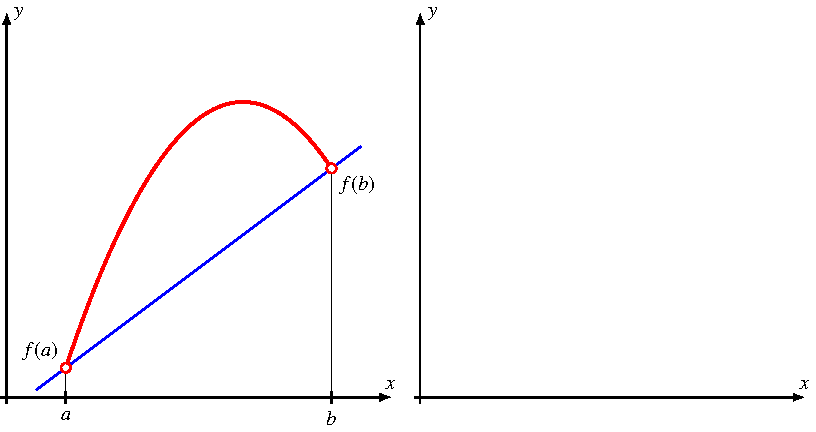
\includegraphics{chapters/30-interpolation/figures/mittelwertsatz.pdf}
\caption{Der Mittelwertsatz~\ref{buch:satz:mittelwertsatz} besagt, dass
die Sekante des Graphen einer differenzierbaren Funktion immer eine
Tangente mit der gleichen Steigung hat.
Diese Eigenschaft kann man auch für eine beliebige ebene Kurven
erwarten (rechts), dies ist der Inhalt des verallgemeinerten
Mittelwertsatzes~\ref{buch:satz:vmittelwertsatz}.
\label{buch:polynome:figure:mittelwertsatz}}
\end{figure}

\begin{satz}[Mittelwertsatz]
\label{buch:satz:mittelwertsatz}
Zu einer auf dem Intervall $[a,b]$ differenzierbaren Funktion $f(x)$ gibt
es immer ein $\xi\in[a,b]$ mit
\[
f'(\xi) = \frac{f(b)-f(a)}{b-a}
\]
(Abbildung~\ref{buch:polynome:figure:mittelwertsatz} links).
\end{satz}

\begin{proof}[Beweis]
Man betrachtet die Funktion 
\[
g(x) = f(x) - \frac{f(b)-f(a)}{b-a}(x-a),
\]
sie hat an den Intervallenden die Werte
\begin{align*}
g(a) &= f(a) - \frac{f(b)-f(a)}{b-a}(a-a)=f(a),
\\
g(b) &= f(b) - \frac{f(b)-f(a)}{b-a}(b-a) = f(b) - \bigl(f(b)-f(a)\bigr) = f(a).
\end{align*}
Die Funktionswerte an den Intervallenden sind also gleich,
nach dem Satz~\ref{buch:satz:rolle} von Rolle hat also
die Ableitung $g'$ eine Nullstelle $\xi\in[a,b]$:
\[
g'(\xi) = f'(\xi) - \frac{f(b)-f(a)}{b-a} = 0
\quad
\Rightarrow
\qquad
f'(\xi) = \frac{f(b)-f(a)}{b-a}.
\qedhere
\]
\end{proof}

\subsubsection{Mittelwertsatz und ebene Kurven}
\index{ebene Kurve}%
\index{Kurve, ebene}%
Die von Abbildung~\ref{buch:polynome:figure:mittelwertsatz} vermittelte
Intuition lässt sich auch für beliebige parametrisierte Kurven
$\gamma\colon[a,b]\to\mathbb R:\to\mapsto (x(t),y(t))$ in der Ebene
verallgemeinern (Abbildung~\ref{buch:polynome:figure:mittelwertsatz} rechts).
Sind die Punkte $A=(x(a),y(a))$ und $B=(y(a),y(b))$ verschieden,
so dass die Richtung von $A$ nach $B$ wohldefiniert ist, dann erwarten
wir einen Zwischenstelle $\xi$ mit einer Tangente mit derselben Richtung.
\index{Tangente}%

\begin{satz}
\label{buch:satz:mittelwertsatz2d}
Sei $\gamma\colon[a,b]\to\mathbb R:t\mapsto (x(t),y(t))$ eine
stetig differenzierbare ebene Kurve mit $|\dot{\gamma}(t)|\ne 0$ für
alle $t\in[a,b]$ und $A=\gamma(a)\ne\gamma(b)=B$.
Dann gibt es ein $\xi\in[a,b]$ derart, dass $\dot{\gamma}(\xi)$ die gleiche
Richtung hat wie $\overrightarrow{AB}$.
\end{satz}

\begin{proof}[Beweis]
Zwei Vektoren haben die gleiche Richtung, wenn die Determinante
mit den Vektoren als Spaltenvektoren verschwindet.
\index{Determinante}%
Der Mittelpunkt der Strecke $AB$ ist
$M=(x_M,y_M) = (\frac12(x(a)+x(b)),\frac12(y(a)+y(b)))$.
Wir definieren die Funktion
\[
h(t)
=
\det(\overrightarrow{M\gamma(t)}, \overrightarrow{AB})
=
\biggl|
\begin{matrix}
x(t) - x_M & x(b)-x(a) \\
y(t) - y_M & y(b)-y(a)
\end{matrix}
\biggr|
\]
Da die Strecken $AB$ und $MA$ bzw.~$MB$ die gleiche Richtung haben,
gilt an den Stellen $t=a$ und $t=b$ 
\[
h(a)
=
\det (\overrightarrow{MA},\overrightarrow{AB})
= 0
\qquad\text{and}\qquad
h(b)
=
\det (\overrightarrow{MB},\overrightarrow{AB})
=
0.
\]
Nach dem Satz von Rolle muss es daher ein $\xi\in[a,b]$ geben mit
\index{Satz von Rolle}%
\begin{equation}
0
=
h'(\xi)
=
\det(
\dot{\gamma}(\xi),
\overrightarrow{AB}
)
=
\biggl|
\begin{matrix}
x'(\xi) & x(b)-x(a) \\
y'(\xi) & y(b)-y(a)
\end{matrix}
\biggr|,
\label{buch:polynome:eqn:mittelwertsatz2d}
\end{equation}
was natürlich wieder bedeutet, dass die Tangente $\dot{\gamma}(\xi)$ 
parallel ist zur Strecke $AB$.
\end{proof}


\begin{satz}[Verallgemeinerter Mittelwertsatz]
\label{buch:satz:vmittelwertsatz}
Sind $x(t)$ und $y(t)$ stetig differenzierbare Funktionen auf dem Intervall
$[a,b]$ derart, dass $x(a)\ne x(b)$ oder $y(a)\ne x(b)$ und ausserdem
$y'(t)\ne 0$ für $t\in[a,b]$.
Dann gibt es ein $\xi\in[a,b]$ mit
\[
\frac{y'(\xi)}{x'(\xi)}
=
\frac{y(b)-y(a)}{x(b)-x(a)}.
\]
\end{satz}

\begin{proof}[Beweis]
Die Bedingungen bedeuten, dass die die Kurve $\gamma(x(t),y(t))$
den Voraussetzungen des Satzes~\ref{buch:satz:mittelwertsatz2d}
genügt.
Es gibt daher einen Punkten $\xi\in[a,b]$ wo die Tangente
parallel zur Strecke $AB$ ist.
Nach~\ref{buch:polynome:eqn:mittelwertsatz2d} bedeutet dies
\[
y'(\xi) \cdot (x(b)-x(a))
-
x'(\xi) \cdot (y(b)-y(a))
=0
\qquad\Rightarrow\quad
\frac{x'(\xi)}{y'(\xi)}
=
\frac{y(b)-y(a)}{x(b)-x(a)}.
\qedhere
\]
\end{proof}

\subsubsection{Mittelwertsatz in $\mathbb R^n$}
\index{Mittelwertsatz in $\mathbb R^n$}
Der Mittelwertsatz verspricht die Existenz eines Arguments $\xi\in[a,b]$,
gibt aber keinerlei Hinweise darauf, wie $\xi$ berechnet werden könnte. 
Ausserdem lässt sich der Satz in dieser Form nicht auf höherdimensionale
Situationen verallgemeinern.
In vielen Anwendungen des Mittelwertsatzes ist der genaue Wert von $\xi$
gar nicht nötig.
Meistens wird nur verwendet, dass die Ableitung eine Abschätzung dafür
gibt, wie gross der Unterschied zwischen $f(b)$ und $f(a)$ sein kann.
\index{Ableitung}%
Dies kann zum Beispiel wie im folgenden Satz formuliert werden.

\begin{satz}
Für eine in $[a,b]$ stetig differenzierbare Funktion
$f\colon [a,b]\to\mathbb R^n$ gibt es ein $\xi\in[a,b]$ mit
\[
|f(b)-f(a)| \le |f'(\xi)|\cdot |b-a|.
\]
\end{satz}

\begin{proof}[Beweis]
\cite[(8.5.1)]{buch:dieudonne}
\end{proof}

Diese Form ist ausreichend, um zum Beispiel Fehlerabschätzungen in der
Numerik durchzuführen.
\index{Fehlerabschätzung}%

\subsubsection{Taylor-Reihe mit Lagrange-Restterm}
\index{Taylor-Reihe}%
\index{Lagrange-Restterm}%
Die Ableitung $f'(a)$ einer Funktion $f(x)$ an der Stelle $a$ ist definiert
als die beste lineare Approximation
\[
f(x) = f(a) + f'(a)\cdot (x-a) + o(|x-a|).
\]
Der Mittelwertsatz besagt, dass
\[
f(x) = f(a) + f'(\xi) \cdot (x-a)
\]
für ein geeignetes $\xi\in[a,x]$.
Man kann also sagen, dass $f(a)$ eine Approximation für $f(x)$ mit einem
Fehler der Form $f'(\xi)\cdot(x-a)$ für ein geeignetes $\xi\in[a,x]$ ist.
Das Taylor-Polynom verallgemeinert diese Beobachtung auf eine Approximation
höherer Ordnung.

\begin{satz}
Sei $f(x)$ eine $n+1$-mal stetig differenzierbare Funktion in einer
Umgebung von $a$.
Dann ist das {\em Taylor-Polynom}
\begin{align*}
T_{a,n}f(x)
&=
f(a) + f'(a)\cdot (x-a) + f''(x)\frac{(x-a)^2}{2!} + f'''(x)\frac{(x-a)^3}{3!}
+\dots+f^{(n)}(a)\frac{(x-a)^n}{n!}
\\
&=
\sum_{k=0}^n
f^{(k)}(a) \frac{(x-a)^k}{k!}
\end{align*}
eine Approximation von $f(x)$ derart, dass
\[
f(a)=T_{a,n}f(a),\quad
f'(a)=T_{a,n}f'(a),\quad
f''(a)=T_{a,n}f''(a),\quad
\dots,\quad
f^{(n)}(a)=T_{a,n}f^{(n)}(a).
\]
Ausserdem gibt es einen Wert $\xi\in[a,x]$ derart, dass der Fehler
\index{Fehler}%
\[
R_{n,a}f(x)
=
f(x) - T_{n,a}f(x)
=
f^{(n+1)}(\xi)\frac{(x-a)^{n+1}}{(n+1)!}
\]
ist.
\end{satz}
\index{Taylor-Polynom}%
$R_{n,a}f(x)$ heisst das {\em Lagrange-Restglied} des Taylor-Polynoms.
\index{Lagrange-Restglied}%

\begin{proof}[Beweis]
Zunächst kann die Behauptung über die Ableitungen von $T_{n,a}f(x)$ durch
die Rechnung
\index{Ableitung}%
\begin{align*}
T_{n,a}f'(x)
&=
f'(a) + f''(a) \cdot (x-a) + f'''(a)\frac{(x-a)^2}{2!} + \dots
&&\Rightarrow&
T_{n,a}f'(a) 
&=
f'(a)
\\
T_{n,a}f''(x)
&=
f''(a) + f'''(a) \cdot (x-a) + \dots
&&\Rightarrow&
T_{n,a}f''(a) 
&=
f''(a)
\\
&\;\vdots&&&&\;\vdots
\\
T_{n,a}f^{(n)}(x)
&=
f^{(n)}(a)
&&\Rightarrow&
T_{n,a}f^{(n)}(a)
&=
f^{(n)}(a)
\end{align*}
direkt bestätigt werden.
Daraus folgt, dass die Funktion $g(x) = f(x) - T_{n,a}f(x)$ die Eigenschaft
\begin{equation}
g(a) = g'(a) = g''(a) = \dots = g^{(n)}(a)=0
\label{buch:taylor:gabl}
\end{equation}
hat.
Es muss als nur gezeigt werden, dass es unter den Voraussetzungen
\eqref{buch:taylor:gabl} eine Zahl $\xi$ gibt derart, dass
\[
g(x) = g^{(n+1)}(\xi)\frac{(x-a)^{n+1}}{(n+1)!}
\]
gilt.
Der Fall $n=0$ ist der Mittelwertsatz~\ref{buch:satz:mittelwertsatz}.
\index{Mittelwertsatz}.

Für $n>0$ kann die Behauptung mit vollständiger Induktion bewiesen werden.
\index{Induktion, vollständige}%
\index{vollständige Induktion}%
Sei also bereits bewiesen, dass für eine Funktion, deren Ableitungen bis
zur Ordnung $n-1$ an der Stelle $a$ verschwinden, eine Zahl $\xi\in[a,x]$
existiert mit
\[
g(x) = g^{(n)}(\xi)\frac{(x-a)^n}{n!}
\]
und müssen jetzt zeigen, dass dies auch für $n+1$ gilt.

Wir müssen $g(x)$ mit $(x-a)^{n+1}$ vergleichen und untersuchen
dazu den Quotienten
\[
\frac{g(x)}{(x-a)^{n+1}}.
\]
Zur Abkürzung schreiben wir $h(x) = (x-a)^{n+1}$, es ist also der
Quotient 
\[
\frac{g(x)}{h(x)}
=
\frac{g(x)-g(a)}{h(x)-h(a)}
\]
zu berechnen.
Nach dem verallgemeinerten Mittelwertsatz~\ref{buch:satz:vmittelwertsatz}
gibt es $\xi_1\in[a,x]$ mit
\index{Mittelwertsatz}%
\[
\frac{g'(\xi_1)}{h'(\xi_1)}
=
\frac{g(x)-g(a)}{h(x)-h(a)}.
\]
Da die Ableitung $h'(x)=(n+1)(x-a)^n$ ist, folgt
\begin{equation}
\frac{g'(\xi_1)}{h'(\xi_1)}
=
\frac{g'(\xi_1)}{(n+1) (\xi_1-a)^n}
=
\frac{g(x)-g(a)}{h(x)-h(a)}
=
\frac{g(x)}{(x-a)^{n+1}}.
\label{buch:taylor:eqn1}
\end{equation}
Die Ableitungen der Ordnung $\le n-1$ der Funktion $g'(x)$ verschwinden
im Punkt $a$, nach Induktionsvoraussetzung gibt es also ein $\xi$ derart,
dass
\index{Induktionsvoraussetzung}%
\[
g'(\xi_1)
=
(g')^{(n)}(\xi) \frac{(\xi_1-a)^{n}}{n!}
=
g^{(n+1)}(\xi)\frac{(\xi_1-a)^n}{n!}
\]
gilt.
Setzt man dies in \eqref{buch:taylor:eqn1} ein, erhält man
\[
\frac{g(x)}{(x-a)^{n+1}}
=
\frac{g'(\xi_1)}{(n+1)(\xi_1-a)^n}
=
g^{(n+1)}(\xi)\frac{(\xi_1-a)^n}{n!} \frac{1}{(n+1)(\xi_1-a)^n}
=
g^{(n+1)}(\xi)\frac{1}{(n+1)!}.
\]
Durch Multiplikation mit $(x-a)^{n+1}$ erhalten wir
\[
g(x) = g^{(n+1)}(\xi)\frac{(x-a)^{n+1}}{(n+1)!}.
\]
Damit ist der Induktionsschritt vollzogen und die Restformel bewiesen.
\index{Induktionsschritt}%
\end{proof}

\begin{beispiel}
Die Funktion $f(x)=x^N$ hat an der Stelle $a=0$ verschwindende
Ableitungen bis zur Ordnung $N-1$.
Das Taylor-Polynom $T_{0,n}f(x)$ der Ordnung $n$ dieser Funktion
verschwindet daher für $n<N$.
\index{Taylor-Polynom}%
Nach der Restformel für das Taylor-Polynom gibt es Zahlen $\xi_n$ derart
\begin{align*}
R_{n,0}f(x)
=
f(x)
&=
x^N
= 
f^{(n+1)}(\xi_n) \frac{x^{n+1}}{(n+1)!}
\\
&=
\frac{
N\cdot(N-1)\cdot(N-2)\cdot\dots\cdot(N-n)
}{
1\cdot 2 \cdot 3 \cdot\dots \cdot (n+1)
}
\xi_n^{N-n-1} 
=
\binom{N}{n+1} \xi_n^{N-n-1}
\\
\Rightarrow\qquad
\xi_n
&=
\binom{N}{n+1}^{\frac{-1}{N-n-1}} x^{\frac{N}{N-n-1}}.
\qedhere
\end{align*}
\end{beispiel}

\subsubsection{Fehlerabschätzungen}
\index{Fehlerabschätzung}%
Im Hinblick auf die nachfolgende Diskussion des Fehlers des
Interpolationspolynoms formulieren wir dies noch als eine
Fehlerabschätzung.
Das Taylor-Polynom approximiert die Funktion $f(x)$ durch ein
Polynom vom Grad $n$.
Der Fehler des Taylor-Polynoms ist
\[
|f(x) - T_{n,a}f(x)|
=
\biggl|
f^{(n+1)}(\xi)
\frac{(x-a)^{n+1}}{(n+1)!}
\biggr|
=
|f^{(n+1)}(\xi)|\cdot
\biggl|
\frac{(x-a)^{n+1}}{(n+1)!}
\biggr|
\le
\max_{\xi\in [a,x]} |f^{(n+1)}(\xi)|
\biggl|
\frac{(x-a)^{n+1}}{(n+1)!}
\biggr|,
\]
er ist also beschränkt einerseits durch ein Polynom mit Grad $n+1$
und den grössten Wert der $(n+1)$-te Ableitung im Intervall $[a,x]$.
Die Fehlerformel für das Interpolationspolynom wird von der genau
gleichen Art sein.
\index{Interpolationspolynom}%

\subsubsection{Fehler des Lagrange-Interpolationspolynoms}
\index{Lagrange-Interpolationspolynom}%
Der folgende Satz gibt vollständige Auskunft über den Fehler des
Interpolationspolynoms.

\begin{satz}
\label{buch:satz:lagrangefehler}
Sei $p$ ein Polynom vom Grad $n$, welches mit der $n+1$-mal differenzierbaren
Funktion $f$ an den $n+1$ Stellen
\[
a = x_0 < x_1 < x_2 < \dots  < x_{n-1} < x_n=b
\]
übereinstimmt.
Dann gibt es für jedes $x\in[a,b]$ ein $\xi_x\in [a,b]$ mit
\begin{equation}
f(x) - p(x) = \frac{f^{(n+1)}(\xi_x)}{(n+1)!} l(x).
\label{buch:equation:polyfehler}
\end{equation}
\end{satz}

\begin{proof}[Beweis]
An den Stützstellen $x_i$ ist $f(x_i)-p(x_i)=0$ und $l(x_i)=0$, die
Gleichung~\eqref{buch:equation:polyfehler} ist also trivialerweise
erfüllt.

Sei jetzt also $x\in[a,b]$ verschieden von allen $x_i$.
Da $l(x)\ne 0$ ist, gibt es eine Zahl $c$ derart, dass
\begin{equation}
f(x)-p(x)=cl(x)
\qquad\Leftrightarrow\qquad
f(x)-p(x)-cl(x)=0.
\label{buch:equation:polyfehler1}
\end{equation}
Die Funktion $g(x)=f(x)-p(x)-cl(x)$ verschwindet in allen Stützstellen $x_i$
und zusätzlich auch noch im Punkt $x$, sie hat also $n+1$ Nullstellen.

Nach dem Nullstellen-Schachtelungssatz~\ref{buch:satz:nullstellen}
hat die $n+1$-te Ableitung von $g$ eine Nullstelle im Intervall.
Es gibt also eine Zahl $\xi_x\in[a,b]$ mit $g^{(n+1)}(\xi_x)=0$.

Da $p$ Grad $n$ hat, ist die $n+1$-te Ableitung $0$.
Das Polynom $l(x)$ hat die Form
\[
l(x) = x^{n+1} -(x_0+x_1+\dots+x_{n-1}+x_n)x^{n-1} + \dots + (-1)^{n+1}x_0x_1\dots x_{n-1}x_n,
\]
seine $n+1$-Ableitung ist die Konstanten $(n+1)!$.

Die Folgerung $g^{(n+1)}(\xi_x)=0$ wird damit zu
\[
0 = f^{(n+1)}(\xi_x) -c (n+1)!
\qquad\Rightarrow\quad
c=\frac{f^{(n+1)}(\xi_x)}{(n+1)!}.
\]
Einsetzen diese Wertes für $c$ in \eqref{buch:equation:polyfehler1} ergibt
\[
f(x)-p(x) = cl(x)=\frac{f^{(n+1)}(\xi_x)}{(n+1)!} l(x),
\]
wie behauptet.
\end{proof}

Dieser Satz erlaubt den Fehler eines Interpolationspolynoms abzuschätzen,
wenn die $n+1$-te Ableitung der Funktion $f$ bekannt ist.
Wir bezeichnen mit
\[
\|g\| = \sup_{a\le x\le b} |g(x)|
\]
die {\em Supremun-Norm} der Funktion $g$ im Intervall $[a,b]$.
\index{Supremum-Norm}

\begin{korollar}
\label{buch:korollar:interpolationsfehler}
Ist $p$ ein Interpolationspolynom vom Grad $n$, welches mit der Funktion
$f$ in den Stellen $a=x_0<x_1<\dots <x_{n+1}<x_n=b$ übereinstimmt, dann
ist 
\[
|f(x)-p(x)| \le \frac{\|f^{(n+1)}\|}{(n+1)!} |l(x)|.
\]
\end{korollar}

Der Fehler des Interpolationspolynoms vom Grad $n$ ist also beschränkt
durch das Polynom $l(x)$ vom Grad $n+1$ und den grössten Wert der
$(n+1)$-ten Ableitung von $f(x)$.

\begin{beispiel}
\begin{figure}
\centering
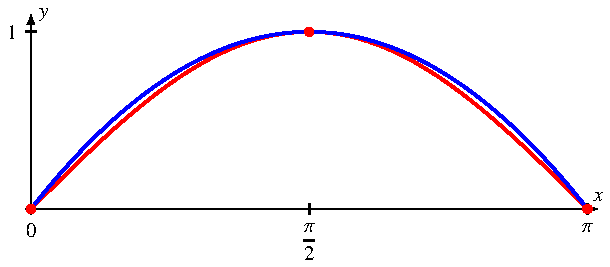
\includegraphics{chapters/30-interpolation/figures/sin.pdf}
\caption{Interpolation der Funktion $f(x)=\sin x$ mit nur drei 
Stützstellen $x_0=0$, $x_1=\frac{\pi}2$ und $x_2=\pi$.
Der Fehler ist deutlich kleiner als die Abschätzung mit
Satz~\ref{buch:satz:lagrangefehler} erwarten lässt.
\label{buch:figure:sin}}
\end{figure}
Die Funktion $f(x)=\sin x$ soll mit den Stützstellen $x_0=0$, $x_1=\frac{\pi}2$
und $x_2=\pi$ interpoliert werden.
Das Interpolationspolynom ist ein quadratisches Polynom mit Nullstellen
$x_0$ und $x_2$, der Funktionswert bei $x_1$ muss $1$ sein.
Man kann sich davon überzeugen, dass das Polynom
\[
p(x) = \frac{4}{\pi^2} x(\pi -x )
\]
diese Eigenschaft hat (Abbildung~\ref{buch:figure:sin}).
Wie gross ist der Fehler dieses Interpolationspolynoms?

Die dritten Ableitungen der Funktion $f(x)=\sin x$ sind, bekannt, es ist
$f^{(3)}(x)=-\cos x$.
Der Betrag von $f^{(3)}(x)$ wird also nie grösser als $1$.
Es folgt, dass
\[
|f(x)-p(x)| \le \frac{1}{3!} l(x)
=
\frac16 |x(x-{\textstyle\frac{\pi}2})(x-\pi)|
\]
Die Ableitung des Polynoms auf der rechten Seite hat Nullstellen bei
$\frac{\pi}2 \pm \frac{\pi}{2\sqrt{3}}$,
durch Einsetzen erhält man den maximalen Wert
\[
\|f^{(3)}\|
=
\frac{\pi^3}{12\sqrt{3}}\approx 1.49179.
\]
Wir schliessen, dass das Interpolationspolynom niemals um mehr als $0.24863$
vom Funktionswert abweichen kann.
\end{beispiel}

%
% Runges Phänomen
%
\subsection{Runges Phänomen
\label{buch:section:interpolation:runge}}
\index{Runge}%
\index{Runges Phänomen}%
Das Korollar~\ref{buch:korollar:interpolationsfehler} besagt, dass der
Fehler des Interpolationspolynom unter anderem durch den Betrag von $l(x)$
begrenzt ist.
Für äquidistante Stützstellen mit Abstand $h$ kann man beobachten,
dass die Oszillationen des Polynoms $l(x)$ gegen den Rand des Intervalls
immer grösser werden.
\index{Oszillation}%
Für einen Punkte in der Mitte jedes Teilintervalls ist $h/2$ der kleinste
mögliche Faktor in $l(x)$. 
Den grössten Faktor findet man für $x$ im ersten oder letzten Teilintervall,
er ist $b-a-h$.
Ausserdem treten mehrere ähnlich grosse Faktoren auf.
Für $x$ in einem Intervall nahe $(a+b)/2$ sind die Faktoren
dagegen nur halb so gross.
Diese Phänomen, dass das die Amplitude der Oszillationen des
Interpolationspolynoms $l(x)$ gegen den Rand des Intervalls immer
grösser wird, ist auch als {\em Runges Phänomen} bekannt.

%
% Tschebyscheff Interpolation
%
\subsection{Wahl der Stützstellen und Tschebyscheff-Interpolationspolynom
\label{buch:section:interpolation:tschebyscheff}}
Die als Runges Phänomen beschriebenen Oszillationen am Rande des Intervalls
können verkleinert werden, wenn man dafür sorgt, dass
mit grösserem Abstand von der Mitte des Intervalls der Abstand der
Stützstellen untereinander ebenfalls verkleinert.
\index{Runges Phänomen}%
\index{Oszillation}%
Dies garantiert, dass neben den grossen Faktoren in der Nähe von $b-a$ 
auch wesentlich kleinere Faktoren auftreten, so dass die extremen Werte
nahe den Intervallenden vergleichbar mit den Werten im Inneren des
Intervalls werden.

\begin{figure}
\centering
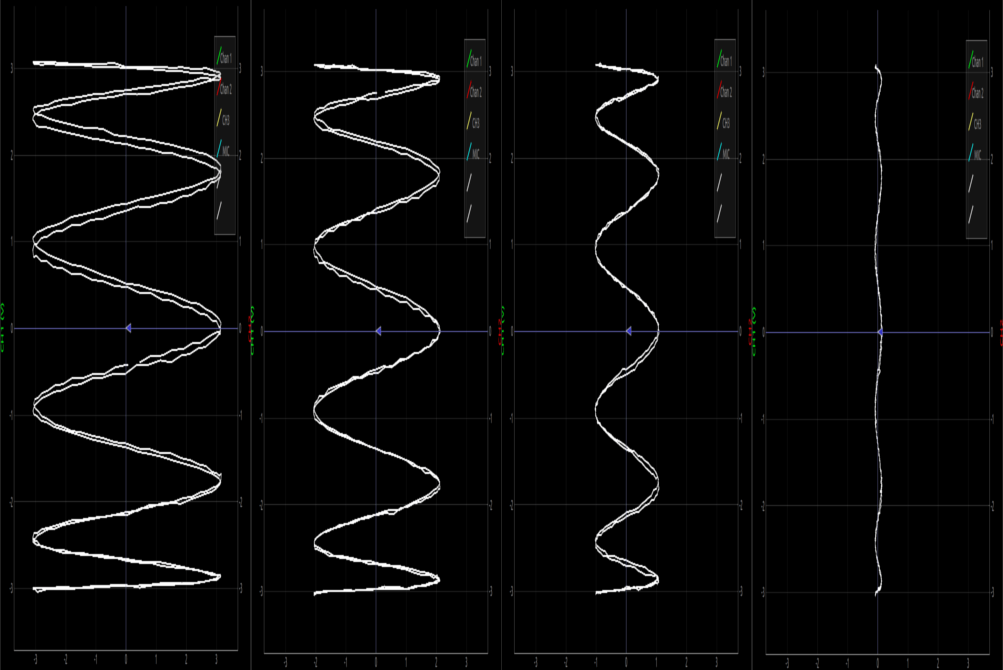
\includegraphics[width=\hsize]{chapters/30-interpolation/figures/lissajous.pdf}
\caption{Diese Lissajous-Figur suggeriert eine mögliche Lösung für eine 
Interpolationspolynom mit besonders kleinem Fehler.
\index{Lissajous-Figur}%
Wenn sich diese Kurve als Polynom ausdrücken lässt, bleibt der Fehler über
das ganze Definitionsintervall gleichmässig beschränkt.
\label{buch:figure:lissajous}}
\end{figure}

\begin{figure}
\centering
\includegraphics[width=\hsize]{chapters/30-interpolation/figures/lissajous-chebyshef.pdf}
\caption{Lissajous-Figur von Abbildung~\ref{buch:figure:lissajous}
mit eingezeichnetem Tschebyscheff-Polynom und Nullstellen
desselben.
\index{Tschebyscheff-Polynom}%
\index{Nullstelle}%
Das Maximum des Betrags des Tschebyscheff-Polynoms ist 1 und liefert 
damit eine obere Schranke für den Fehler des zugehörigen
Interpolationspolynoms.
\index{Fehler}%
\label{buch:figure:lissajous-chebyshef}}
\end{figure}

Die beste Approximation durch ein Interpolationspolynom kann man also
erwarten, wenn $l(x)$ im Intervall $[a,b]$ keine besonders grossen Werte
annimmt.
\index{Approximation}%
Eine Funktion ähnlich wie $\sin x$ oder $\cos x$, die unendlich viele
Extremewerte $\pm 1$ haben, würde dieses Kriterium erfüllen, aber
$\sin x$ und $\cos x$ sind keine Polynome.
Sie sind auch auf auf einem viel grösseren Intervall als nötig definiert,
nämlich ganz $\mathbb R$.
Ein verwandtes Beispiel sind Lissajous-Figuren.
\index{Lissajous-Figur}%
Abbildung~\ref{buch:figure:lissajous} suggeriert, dass eine geeignete
Lissajous-Figur als Graph für ein Interpolationspolynom mit sehr
geringem Fehler dienen könnte, wenn man sie als Polynom darstellen kann.
Eine solche Lissajous-Figur entsteht als Kurve
$\gamma_n\colon t\mapsto (\cos t, \cos nt)$ oder eine anderes trigonometrisches
Polynom als zweite Komponente.
\index{trigonometrisches Polynom}%
\index{Polynom!trigonometrisch}%
Die Abbildung~\ref{buch:figure:lissajous-chebyshef} zeigt diese Kurve
$\gamma_n(t)$
für den Fall $n=13$ der Lissajous-Figur von
Abbildung~\ref{buch:figure:lissajous} überlagert.
Die gute Übereinstimmung bestätigt die obige Beobachtung.

\subsubsection{Die Tschebyscheff-Polynome}
Es stellt sich also die Frage, ob $\cos nt$ als Polynom in $z=\cos t$
ausgedrückt werden kann.
Sei also
\[
T_n(x)
=
T_n(\cos t)
= 
\cos nt.
\]
Für kleine $n$ kann man unmittelbar verifizieren, dass $T_n(z)$ ein
Polynom ist:
\begin{equation}
\begin{aligned}
T_0(x) &= 1,\\
T_1(x) &= x,\\
T_2(x) &= \cos 2t = 2\cos^2 t-1 = 2x^2 -1
\quad\text{und}
\\
T_3(x) &= \cos 3t = 4\cos^3 t - 3\cos t = 4x^3-3x.
\end{aligned}
\label{buch:tschebyscheff:erste}
\end{equation}
Für kleine Werte von $n$ ist also direkt nachprüfbar, dass $T_n(x)$
ein Polynom ist.

Wir benötigen eine Formel, mit der sich Werte der Polynome $T_n(x)$
effizient berechnen lassen, ohne dass das Polynom in expliziter
Form ermittelt werden muss.
Im Folgenden soll dazu eine Rekursionsformel hergeleitet werden.
\index{Rekursionsformel}%

Aus den Additionstheoremen für den Kosinus folgt die Formel für die
Summe von zwei Konsinus-Funktionen
\index{Additionstheorem}%
\begin{align}
\cos (n+1)t + \cos(n-1)t
&=
2 \cos \frac{(n+1)t + (n-1)t}2 \cos \frac{(n+1)t -(n-1)t}2
=
2\cos nt \cos t
\notag
\\
T_{n+1}(x)+T_{n-1}(x)&=2T_n(x)x
\notag
\\
T_{n+1}(x) &= 2xT_n(x) - T_{n-1}(x).
\label{buch:tschebyscheff:rekursion}
\end{align}
Wenn $T_n(x)$ und $T_{n-1}(x)$ Polynome sind, dann ist auch $T_{n+1}(x)$
ein Polynom.
Aus den bereits bekannten Polynomen~\eqref{buch:tschebyscheff:erste} und
der Rekursionsformel~\eqref{buch:tschebyscheff:rekursion} folgt jetzt mit
vollständiger Induktion, dass alle $T_n(x)$ Polynome sind.
\index{Induktion}%
\index{vollständige Induktion}%
Sie heissen {\em Tschebyscheff-Polynome}.
\index{Tschebyscheff-Polynom}%
Die Rekursionsformel kann dazu verwendet werden, die Polynome explizit
zu berechnen.
Zum Beispiel folgt für die nächsten drei Polynome
\begin{align*}
T_4(x) &= 8x^4-8x^2 + 1,
\\
T_5(x) &= 16x^5-20x^3+5x \quad\text{und}
\\
T_6(x) &= 32x^6-48x^4+18x^2-1.
\end{align*}
Da das Interpolationspolynom den führenden Koeffizienten $1$ haben muss,
muss $l(x) = 2^{1-n}T_n(x)$ gewählt werden.

\subsubsection{Tschebyscheff-Stützstellen}
\index{Tschebyscheff-Stützstellen}%
Die Polynome $T_n(x)$ sind eigentlich nicht nötig, da für die Konstruktion
des Interpolationspolynoms nur die Nullstellen nötig sind.
Wegen $T_n(x)=\cos nt$ liegt eine Nullstelle genau dann vor, wenn
$nt = \frac{\pi}2 + k\pi$, $k\in\mathbb Z$.
Die zugehörigen Werte von $z$ sind
\[
x_k
=
\cos t = \cos\frac{\pi(2k+1)}{2n}.
\]
In Abbildung~\ref{buch:figure:tschebyscheff-vergleich} sind 
die Polynome $2^{n-1}l(x)$ vom Grad $n$ oben für äquidistante Stützstellen
und unten für Tschebyscheff-Stützstellen im Vergleich dargestellt.
Wie in der Einleitung zu diesem Abschnitt angekündigt, oszillieren die
Polynome für äquidistante Stütztstellen nahe den Intervallenden.
\index{Oszillation}%
Für Tschebyscheff-Stützstellen wird $2^{n-1}l(x)$ betragsmässig nie
grösser als $1$.
\begin{figure}
\centering
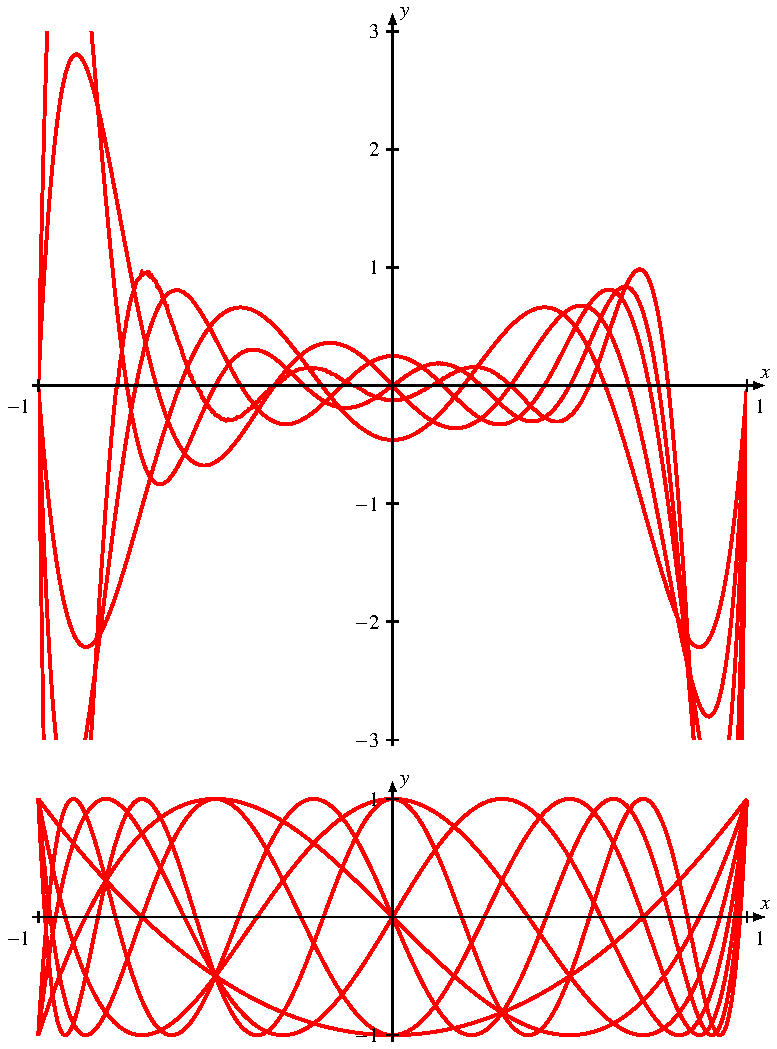
\includegraphics{chapters/30-interpolation/figures/vergleich.pdf}
\caption{Vergleich der Oszillationen bei äquidistanten Stützstellen (oben)
und bei Tschebyscheff-Stützstellen.
Damit die Abweichungen sichtbar werden, sind die Polynome $l(x)$ vom Grad
$n$ mit dem Faktor $2^{n-1}$ skaliert.
Bei Verwendung von Tscheby\-scheff-Stützstellen wächst $2^{n-1}l(x)$
nie über $1$ an, während bei äquidistanten Stützstellen die in der
Einleitung zu diesem Abschnitt diskutierten Oszillationen nahe den
Intervallenden auftreten.
\label{buch:figure:tschebyscheff-vergleich}}
\end{figure}

\begin{figure}
\centering
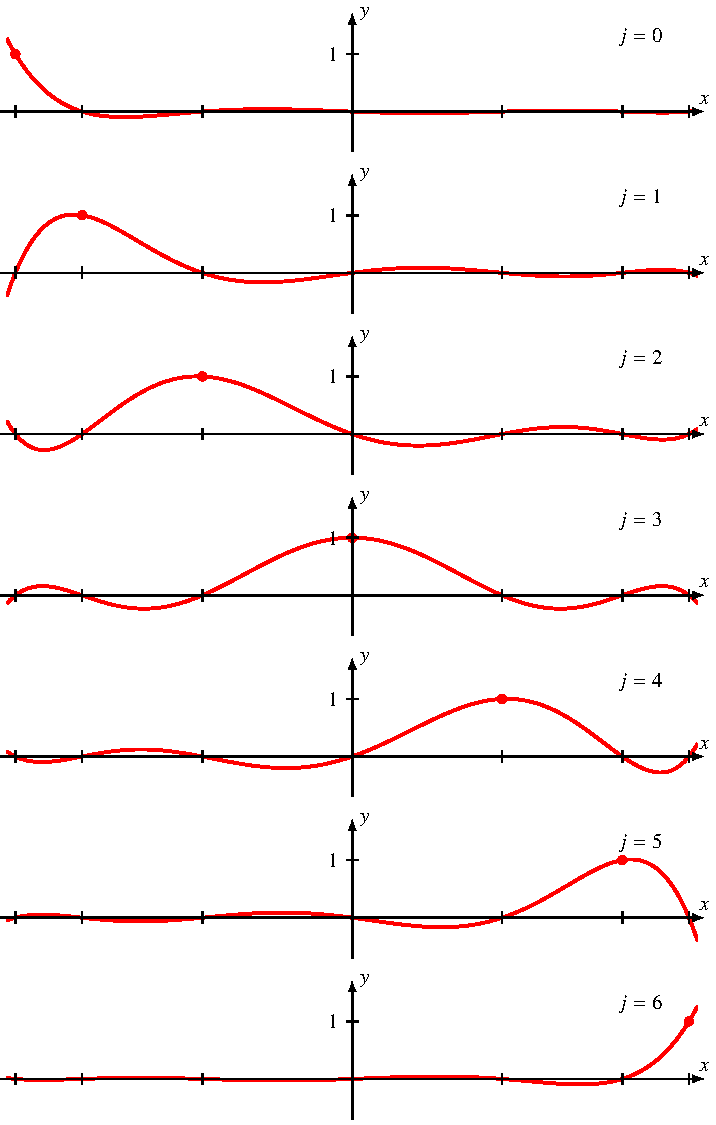
\includegraphics{chapters/30-interpolation/figures/tschebasis.pdf}
\caption{Basisinterpolationspolynome vom Grad 7 für
Tschebyscheff-Stützstellen
\label{buch:figure:tschebyscheffbasis}}
\end{figure}
Abbildung~\ref{buch:figure:tschebyscheffbasis} zeigt die Basispolynome
vom Grad 7 $l_j(x)$ für Tschebscheff-Stütztstellen.
Da bei Verwendung von Tschebyscheff-Stützstellen die Polynome $l(x)$
keine ausgeprägten Oszillationen an den Intervallenden aufweisen, 
sind auch die Basispolynome $l_j(x)$ vor allem in der Nähe der
jeweiligen Stützstelle $x_j$ wesentlich von $0$ verschieden.


%
% normal.tex
%
% (c) 2020 Prof Dr Andreas Müller, Hochschule Rapperswil
%
\subsubsection{Vergleich der Fehler}
In diesem Abschnitt vergleichen wir die Fehler der Interpolationspolynome
für die Funktion
\index{Standardnormalverteilungsdichte}%
\index{Normalverteilung}%
\[
f(x)
=
\frac{1}{\sqrt{2\pi}} e^{-x^2/2}
\]
nach Lagrange mit äquidistanten Stützstellen und mit
\index{äquidistante Stützstellen}%
\index{Stützstellen!äquidistant}%
Tschebyscheff-Stützstellen.
\index{Tschebyscheff-Stützstellen}%

\begin{figure}
\centering
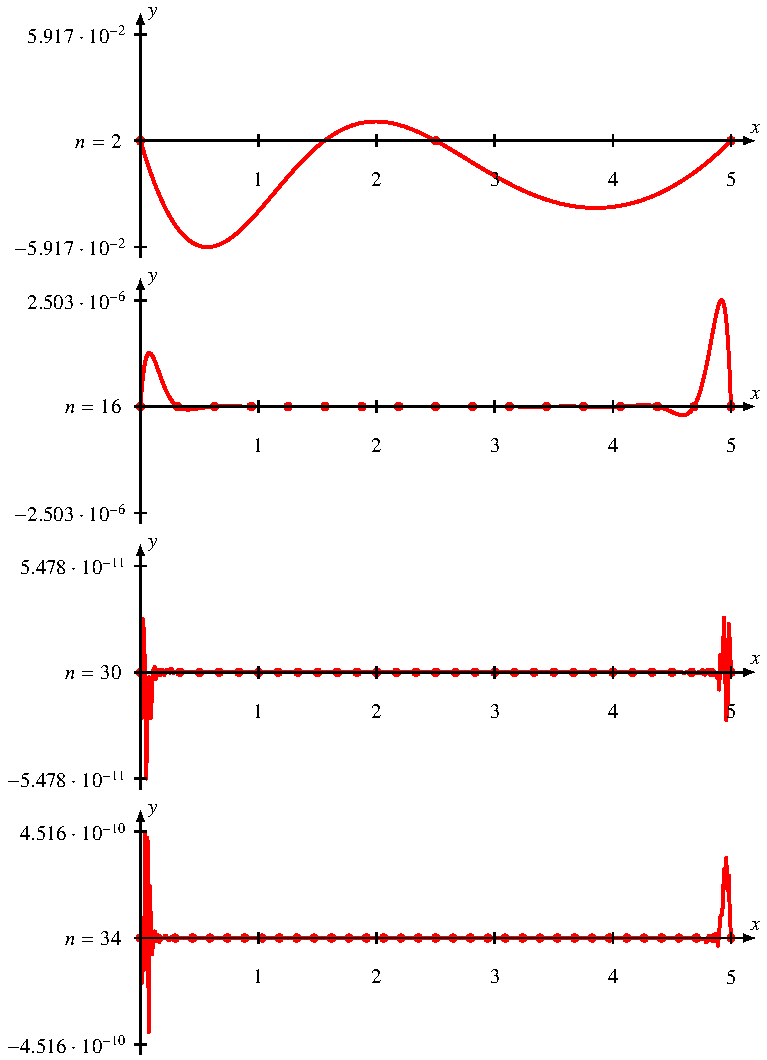
\includegraphics{chapters/30-interpolation/figures/norm.pdf}
\caption{Fehler des Lagrange-Interpolationspolynoms für die Funktion
$f(x)=e^{-x^2/2}/\sqrt{2\pi}$.
Der Fehler nimmt mit der Anzahl der Stützstellen bis $n=30$ ab, danach
wird die Berechnung instabil und der Fehler nimmt wieder zu.
\index{instabil}%
\label{buch:figure:lagrangefehler}}
\end{figure}


\begin{figure}
\centering
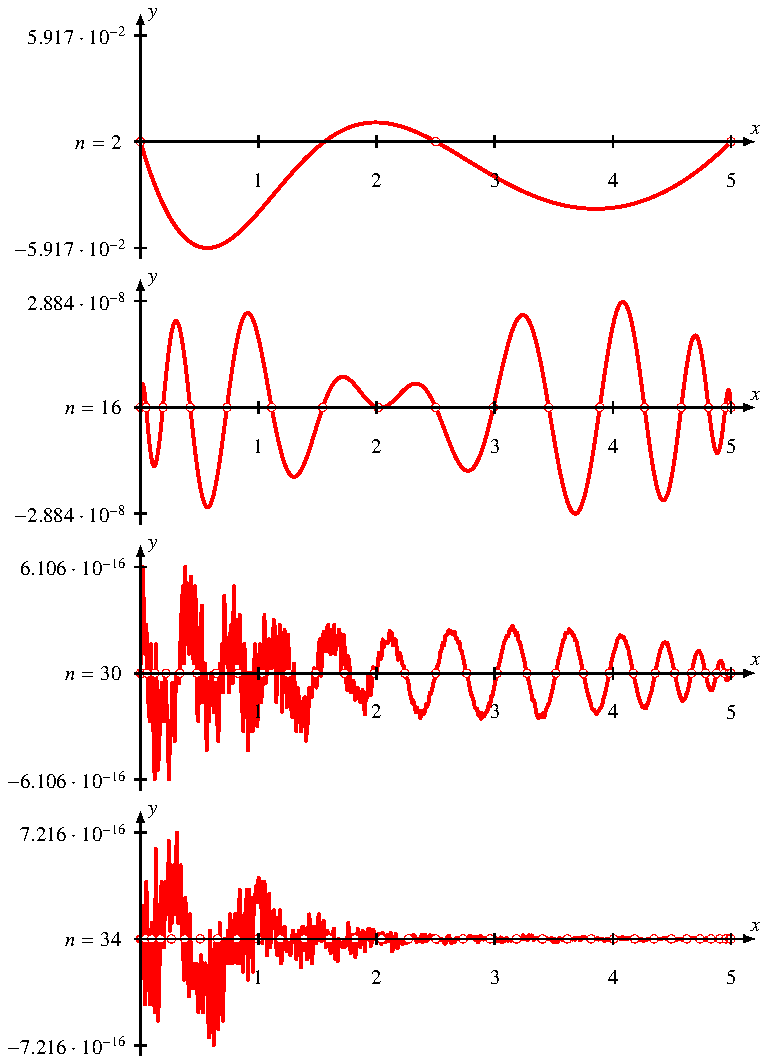
\includegraphics{chapters/30-interpolation/figures/tscheb.pdf}
\caption{Fehler des Interpolationspolynomes für die Funktion
$f(x)=e^{-x^2/2}/\sqrt{2\pi}$ mit Stützstellen nach Tschebyscheff.
Der Fehler bleibt über das ganze Intervall gleichmässig.
Für eine grosse Zahl von Stützstellen erreicht die Interpolation die
Maschinengenauigkeit.
\label{buch:figure:tschebyschefffehler}}
\end{figure}

Die Resultate sind in Abbildung~\ref{buch:figure:lagrangefehler}
für das Lagrange-Interpolationspolynom und
Abbildung~\ref{buch:figure:tschebyschefffehler}
für das Tschebyscheff-Interpolationspolynom dargestellt.
In beiden Abbildungen wird die gleiche Anzahl Stützstellen verwendet.
Beim Lagrange-Interpolationspolynom nimmt der Fehler zunächst schnell ab.
Er ist, wie das Runge Phänomen erwarten lässt, immer am grössten im
äussersten Teilintervall.
Für grösser werdende Anzahl von Stützstellen wird die Berechnung des 
Interpolationspolynoms in diesen äussersten Teilintervallen instabil
und wächst zum Beispiel von $n=30$ zu $n=34$ um eine Grössenordnung an.
Für eine grosse Zahl von Stützstellen kann das Lagrange-Interpolationspolynom
also mindestens am Rand des Intervalls keine zuverlässigen Approximation sein.

Die Verwendung von Tschebyscheff-Stützstellen verbessert die Genauigkeit
schon bei $n=16$ Stützstellen um zwei Grössenordnungen.
Aussserdem sind die Fehler über das ganze Intervall gleichmässig
verteilt.
Bei einer grösseren Anzahl von Stützstellen scheint der Fehler 
vor allem linken Rand stark anzuwachsen.
Da die Funktionswerte aber ungefähr $1$ sind, ist
ein Fehler von $10^{-16}$ genau der typische Rundungsfehler des
\texttt{double} Datentyps.
Man sieht hier als nicht den Fehler des Interpolationspolynoms sondern
die Grenzen der Maschinengenauigkeit.












%
% hermite.tex
%
% (c) 2020 Prof Dr Andreas Müller, Hochschule Rapperswil
%
\section{Hermite-Interpolation
\label{buch:section:hermite}}
\rhead{Hermite-Interpolation}
Das Lagrange-Interpolationspolynom nimmt zwar in umittelbarer Nähe der 
Stützstellen zuverlässig Funktionswerte nahe den gegeben Werten an,
doch insbesondere gegen den Rand des Intervalls können die oft beobachteten
Oszillationen eine schlechte Approximation bewirken.
\index{Lagrange-Interplationspolynom}%
\index{Oszillation}%
\index{Approximation}%
Im Gegensatz zur Taylor-Reihe, deren Ableitung mindestens in der Nähe des
Entwicklungspunktes auch mit der Ableitung der zu approximierenden
Funktion übereinstimmt, gibt es für das Interpolationspolynom keine
solche Garantie.
\index{Taylor-Reiher}%
Beide Schwierigkeiten könnten gemildert werden, indem gefordert wird,
dass das Polynom nicht nur die gleichen Funktionswerte, sondern auch
die gleichen Ableitungen bis zu einer bestimmten Ordnung haben soll.
Dies ist die Idee der {\em Hermite-Interpolation},
\index{Hermite-Interpolation}%
die in diesem Abschnitt vorgestellt werden soll.

%
% Aufgabenstellung
%
\subsection{Aufgabenstellung
\label{b8ch:subsection:hermite:aufgabe}}
Das Hermite-Interpolationspolynom löst die folgende Approximationsaufgabe.

\begin{aufgabe}[Hermite-Interpolationspolynom]
\index{Hermite-Interpolationsproblem}%
\index{Hermite-Interpolationspolynom}%
Gegeben Stützstellen
\[
a=x_0<x_1<x_2<\dots < x_{n-1}<x_n=b
\]
und Funktionswerte $f_i$, $0\le i\le n$, und Werte
$s_i^{(k)}$ der $k$-ten Ableitungen bis zur $m$-ten Ordnung, $1\le k\le m$,
finde ein Polynom $h$, mit
\begin{equation}
h(x_i) = f_i,\quad h^{(k)}(x_i)=s_i^{(k)},\quad 0\le i \le n, 1\le k\le m.
\label{buch:equation:hermitebedingungen}
\end{equation}
\end{aufgabe}
Die Aufgabenstellung formuliert $N=(n+1)(k+1)$ Bedingungen für das Polynom $h$,
es braucht also im Allgemeinen ein Polynom mindestens vom Grade $N=(n+1)(k+1)$,
um alle diese Bedingungen erfüllen zu können.
Ein elementarer Ansatz könnte sein, eine Polynom in der Form
$a_Nx^N+a_{N-1}x^{N-1}+\dots+a_1x+a_0$ anzusetzen, die Bedingungen
\eqref{buch:equation:hermitebedingungen} als lineare Gleichungen für
die Koeffizienten auszuschreiben und das Gleichungssystem zu lössen.
Dieses Vorgehen ist allerdings sehr aufwendig und numerisch nicht besonders
stabil.
Ein Weg analog zur Bestimmung des Lagrange-Interpolationspolynomes in
Abschnitt~\ref{buch:section:interpolation:bestimmung}
ist daher angezeigt.

%
% Bestimmung des Hermite-Interpolationspolynoms
%
\subsection{Bestimmung des Hermite-Interpolationspolynom
\label{buch:subsection:hermite:bestimmung}}
Wir führen die Konstruktion nur für den Fall $m=1$ durch, also für 
Interpolationspolynome, die den Funktionswerten und ersten Ableitungen
übereinstimmen.
Wie in Abschnitt~\ref{buch:section:interpolation:bestimmung} suchen
wir zunächst wieder eine Lösung des folgenden
{\em speziellen Interpolationsproblems}.

\begin{aufgabe}[Spezielles Hermite-Interpolationsproblem]
\index{spezielles Hermite-Interpolationsproblem}%
\index{Hermite-Interpolationsproblem!spezielles}%
Gegeben Stützstellen
\[
a=x_0<x_1<x_2<\dots < x_{n-1}<x_n=b
\]
finde Polynome $h_j$ und $h_j^1$ vom Grad höchstens $2n+1$ derart, dass
\[
\left.
\begin{aligned}
h_j(x_i)&=\delta_{ij}\\
h_j'(x_i)&=0
\end{aligned}\right\}\forall i,j
\qquad\text{und}\qquad
\left.
\begin{aligned}
h_j^1(x_i)&=0\\
h_j^{1\prime}(x_i)&=\delta_{ij}
\end{aligned}\right\}\forall i,j
\]
\end{aufgabe}

\begin{proof}[Lösung]
Ein Polynom vom Grad $2n+2$, welches in allen Stützstellen eine 
doppelte Nullstelle hat, ist das Produkt
\[
(x-x_0)^2 (x-x_1)^2 (x-x_2)^2 \dots (x-x_{n-1})^2 (x-x_n)^2.
\]
Die gesuchten Polynome $h^1_j$ haben in jeder Stützstelle ausser in $x_j$
ein doppelte Nullstelle, die Nullstelle in $x_j$ muss einfach sein.
Ein solches Polynom kann man erhalten, indem man einen der
Faktoren $(x-x_j)$ weglässt, oder zu
\[
p_j(x)
=
(x-x_0)^2 (x-x_1)^2 \cdots \widehat{(x-x_k)^2} \dots (x-x_{n-1})^2(x-x_n)^2
\]
einen solchen Faktor hinzufügt:
\[
h_j^1(x)
=
c_j^2 (x-x_j) p_j(x),
\]
die Konstante $c_j^2$ muss passend gewählt werden, damit die Ableitung
\[
h_j^{1\prime}(x)
=
c_j^2 \underbrace{\frac{d}{dx}(x-x_j)}_{\displaystyle=1}
+
c_j^2
(x-x_j)
\frac{d}{dx} p_j(x)
\]
den richtigen Wert bekommt.
An der Stelle $x=x_j$ fällt der zweite Term weg und es bleibt
\[
h_j^{1\prime}(x_j)
=
c_j^2 p_j(x_j).
\]
und damit ist $c_j^2 = 1/p_j(x_j)$.
Dies ist das Quadrat des entsprechenden Normierungsfaktors, der beim
Lagrange-Interpolationspolynom zur Anwendung kam.

Die Polynome $h_j$ haben in allen Stützstellen ausser $x_j$ eine doppelte
Nullstelle.
Das Produkt $p_j(x)$ teilt diese Eigenschaft.
Da es vom Grad $2n$ ist, haben wir nur die Freiheit, einen Linearfaktor
der Form $(u_j(x-x_j)+v_j)$ hinzuzufügen, um $h_j$ zu erhalten.
Es müssen also $u_j$ und $v_j$ so gewählt werden, dass für
\begin{equation}
h_j(x)=(u_j(x-x_j)+v_j) p_j(x)
\qquad
\text{die Gleichungen}
\qquad
\left\{
\quad
\begin{aligned}
h_j(x_j) &= v_j p_j(x_j) = 1\\
h'_j(x_j) &= u_j p_j(x_j) + v_j p'_j(x_j)=0
\end{aligned}
\right.
\label{buch:equation:hermite:4711}
\end{equation}
gelten.
Aus der ersten Gleichung folgt $ v_j = 1/p_j(x_j) = c_j^2$, aus der zweiten
\[
u_j
=
-\frac{p'_j(x_j)}{p_j(x_j)^2}
=
- c_j^4 p'_j(x_j).
\]
Einsetzen in die \eqref{buch:equation:hermite:4711} ergibt
\[
h_j(x) = \biggl(-
\frac{p'_j(x_j)}{p_j(x_j)^2} (x-x_j) + \frac{1}{p_j(x_j)}\biggr) p_j(x)
=
\frac{p'_j(x_j)(x-x_j) + p_j(x_j)}{p_j(x_j)^2}p_j(x)
\]
Andererseits ist $p_j(x)(x-x_j)=h^1_j(x)/c_j^1$, man kann also auch
\begin{equation}
h_j(x)  
=
\frac{p_j(x)}{p_j(x_j)}
-
\frac{p'_j(x_j)}{c_j^1p_j(x_j)^2} h_j^1(x)
\label{buch:equation:hermite:4712}
\end{equation}
schreiben.
Der erste Term in~\eqref{buch:equation:hermite:4712} ist das Quadrat
des Lagrange-Interpolationspolynoms $l_j(x)$. 
\end{proof}

Mit der Lösung des speziellen Interpolations-Problems findet man jetzt
auch eine Lösung für das allgemeine Problem.
Das gesuchte Interplationspolynom ist
\[
h(x) 
=
\sum_{j=0}^n f_j h_j(x)
+
\sum_{j=0}^n s_j h^1_j(x).
\]

\subsection{Zwei Stützstellen
\label{buch:subsection:hermite:zweistuetzstellen}}
Der Fall zweier Stützstellen $x_0$ und $x_1$ ist von einiger praktischer
Bedeutung.
Er wird zum Beispiel im Abschnitt~\ref{buch:section:spline}
zum Einsatz kommen.
Die Polynome $h$ und $h^1$ sollen daher für diesen Falll explizit
berechnet werden.

Die Polynome $p_0$ und $p_1$ sind
\[
p_0(x) = (x-x_1)^2
\qquad\text{und}\qquad
p_1(x) = (x-x_0)^2,
\]
woraus $c_0^2 = c_1^2 = (x_1-x_0)^2$ folgt.

Die Polynome $h_0^1$ und $h_1^1$ entstehen durch geeignete Normierung
der Polynome $(x-x_0)p_0(x)$ und $(x-x_1)p_1(x)$, also
\[
h_0^1(x)
=
\frac{(x-x_0)(x-x_1)^2}{(x_0-x_1)^2}
\qquad\text{beziehungsweise}\qquad
h_1^1(x)
=
\frac{(x-x_0)^2(x-x_1)}{(x_0-x_1)^2}.
\]

Für die Polynome $h^1_0$ und $h^1_1$ sind die Konstaten $u_0$ und $u_1$
zu bestimmen.
Die Ableitung der Polynome $p_j$ sind
\[
p_0'(x) = 2(x-x_1)
\qquad\text{und}\qquad
p_1'(x) = 2(x-x_0)
\]
und damit ist
\[
u_0
=
-\frac{p_0'(x_0) }{(x_0-x_1)^4}
=
-2\frac{x_0-x_1}{(x_0-x_1)^4}
=
-\frac{2}{(x_0-x_1)^3}
\qquad\text{und}\qquad
u_1
=
-\frac{p_1'(x_1) }{(x_0-x_1)^4}
=
\frac{2}{(x_0-x_1)^3}.
\]
Aus \eqref{buch:equation:hermite:4711} folgt jetzt
\begin{align*}
h_0(x)
&=
(u_0(x-x_0)+v_0)(x-x_1)^2
=
-\frac{2}{(x_0-x_1)^3}(x-x_0)(x-x_1)^2 + \frac{(x-x_1)^2}{(x_0-x_1)^4}
\\
h_1(x)
&=
(u_1(x-x_1)+v_1)(x-x_0)^2
=
\frac{2}{(x_0-x_1)^3}(x-x_1)(x-x_0)^2 +\frac{(x-x_0)^2}{(x_0-x_1)^2}.
\end{align*}

\subsubsection{Der Spezialfall $x_0=0$}
In diesem Fall schreiben wir $m=x_1$ für die Intervalllänge und erhalten
die Polynome
\begin{equation}
\begin{aligned}
h_0^1(x) &= \frac{x(x-m)^2}{m^2}
&&&
h_1^1(x) &= \frac{x^2(x-m)}{m^2}
\\
h_0(x)   &= \frac{2x(x-m)^2}{m^3} +\frac{(x-m)^2}{m^4}
&&&
h_1(x)   &= -\frac{2x^2(x-m)}{m^3} +\frac{x^2}{m^4}.
\end{aligned}
\end{equation}
\index{$h_0^1(x)$}%
\index{$h_1^1(x)$}%
\index{$h_0(x)$}%
\index{$h_1(x)$}%

\subsubsection{Der Spezialfall $x_0=0$, $x_1=1$}
\begin{figure}
\centering
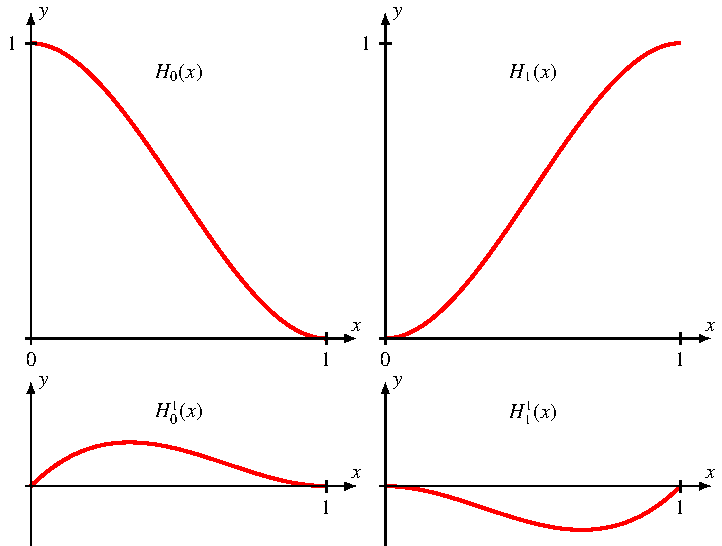
\includegraphics{chapters/30-interpolation/figures/h.pdf}
\caption{Hermite-Basispolynome für das Intervall $[0,1]$
nach \eqref{buch:equation:hermite:h}
\label{buch:figure:hermite:h}}
\end{figure}
Eine besonders einfache Form nehmen die Polynome $h_j^0$ und $h_j^1$ an,
wenn man sie auf das Intervall $[0,1]$ spezialisiert.
Wir bezeichnen diese Polynome mit grossen Buchstaben, sie sind
\begin{equation}
\begin{aligned}
H_0^1(x) &= x(1-x)^2=x^3-2x^2+x
&&&
H_1^1(x) &= (1-x)x^2=x^3-x^2
\\
H_0(x)   &= (1+2x)(1-x)^2= 2x^3-3x^2+1
&&&
H_1(x)   &= (3-2x)x^2 = -2x^3+3x^2
\end{aligned}
\label{buch:equation:hermite:h}
\end{equation}
\index{$H_0^1(x)$}%
\index{$H_1^1(x)$}%
\index{$H_0(x)$}%
\index{$H_1(x)$}%
Graphen dieser Polynome sind in Abbildung~\ref{buch:figure:hermite:h}
dargestellt.

Diese Polynome können auch verwendet werden, die Polynome für ein
beliebiges Intervall wieder zu gewinnen.
Dazu setzen wir $x=(x-x_0)/m$ in die Polynome ein.
Die Polynome $h_0(x)=H_0((x-x_0)/m)$ und $h_1(x)=H_1((x-x_0)/m)$
haben die Werte
\[
\begin{aligned}
h_0(x)
&=
H_0((x-x_0)/m)\bigg|_{x=x_0}
=
H_0(0)=1
&&\text{und}&
h_0(x)
&=
H_0((x-x_0)/m)\bigg|_{x=x_1}
=
H_0(1)=0
\\
h_1(x)
&=
H_1((x-x_0)/m)\bigg|_{x=x_0}
=
H_1(0)=0
&&\text{und}&
h_1(x)
&=
H_1((x-x_0)/m)\bigg|_{x=x_1}
=
H_1(1)=1
\end{aligned}
\]
und Ableitungen
\begin{align*}
h''_i(x_0)
&=
\frac{d}{dx} H_i((x-x_0)/m)\bigg|_{x=x_0}
=
H'_i((x-x_0)/m) \frac{1}{m}\bigg|_{x=x_0}
=
\frac{H_i'(0)}{m} = 0
\end{align*}
an den Intervallenden.

Tun wir dasselbe für die Polynome $H_0^1$ und $H_1^1$, erhalten wir
\begin{align*}
h_j^{1\prime}(x_i)
&=
\frac{d}{dx} H_j^1((x-x_0)/m) \bigg|_{x=x_i}
=
H_j^{1\prime}((x-x_0)/m)\bigg|_{x=x_i} \frac{1}{m}
=
\frac1m
H_j^{1\prime}(i)
=
\frac1m\delta_{ij},
\end{align*}
dies ist bis auf den Faktor $1/m$ korrekt.
Daraus lesen wir ab, dass wir die Polynome
\[
h_j^1(x)
=
mH_j^1((x-x_0)/m)
\]
für die Ableitungen verwenden müssen.

\subsubsection{Zweite Ableitungen}
\index{zweite Ableitung}%
\index{zweite Ableitung!des Hermite-Interpolationspolynoms}%
\index{Hermite-Interplationspolynom!zweite Ableitung}%
Für die spätere Anwendung bei der Spline-Interpolation untersuchen
wir auch noch die zweiten Ableitung des Hermite-Interpolationspolynoms
im Fall zweier Stützstellen am Rande des Intervalls.
Wir tun dies für die Polynome~\eqref{buch:equation:hermite:h}
und kümmern uns später darum, was auf anderen Intervallen passiert.
Wir erhalten die Werte
\[
\begin{aligned}
H_0''(0)                &= -6 &&&  H_0''(1)                &=  \phantom{-}6
\\
H_1''(0)                &=\phantom{-}6 &&&  H_1''(1)       &= -6
\\
H_0^{1\prime\prime}(0)  &= -4 &&&  H_0^{1\prime\prime}(1)  &=  \phantom{-}2
\\
H_1^{1\prime\prime}(0)  &= -2 &&&  H_1^{1\prime\prime}(1)  &=  \phantom{-}4.
\end{aligned}
\]
Unter Verwendung der Substition $x\to (x-x_0)/m$ können wir jetzt auch
die Werte für die zweiten Ableitungen an den Intervallenden für $h_j$ und
$h^1_j$ bestimmen.
Dazu berechnen wir erst die zweite Ableitung einer Funktion $f((x-x_0)/m)$:
\[
\frac{d^2}{dx^2} f((x-x_0)/m)
=
\frac{d}{dx} f'((x-x_0)/m) \frac1m
=
f''((x-x_0)/m) \frac1{m^2}.
\]
Angewendet auf die oben gefundenen Polynome bedeutet dies, 
\[
\begin{aligned}
h_0''(x_0) &=          - 6/m^2
&&\text{und}&
h_0''(x_1) &= \phantom{-}6/m^2 \\
h_1''(x_0) &= \phantom{-}6/m^2
&&\text{und}&
h_1''(x_1) &=          - 6/m^2 \\
h_0^{1\prime\prime}(x_0) &=           -4/m
&&\text{und}&
h_0^{1\prime\prime}(x_1) &= \phantom{-}2/m \\
h_1^{1\prime\prime}(x_0) &=          - 2/m
&&\text{und}&
h_1^{1\prime\prime}(x_1) &= \phantom{-}4/m.
\end{aligned}
\]







%
% bary.tex
%
% (c) 2020 Prof Dr Andreas Müller, Hochschule Rapperswil
%
\section{Baryzentrische Formeln für Interpolationspolynome
\label{buch:section:baryzentrisch}}
\index{baryzentrische Formel}%
Die Interpolationspolynome von Lagrange und Hermite haben 
in der bis jetzt gezeigten Form das folgende grundlegende Problem.
Sie sind definiert über das Produkt
\[
l(x)
=
(x-x_0)(x-x_1)\dots (x-x_{n-1})(x-x_n).
\]
Ist die Zahl der Stützstellen gross und erstrecken sich die 
Stützstellen über einen grossen Bereich, dann sind einzelne Faktoren
$(x-x_i)$ immer gross, wie wir bei der Diskussion von Runges Phänomen
bereits diskutiert haben.
\index{Runges Phänomen}%
Zudem tritt bei der Berechnung eines Wertes in inmittelbarer 
Nähe der Stützstelle $x_j$ in dem Faktor $(x-x_j)$ Auslöschung auf.
Der grosse relative Fehler dieses Faktors wird durch die anderen Faktoren
zu einem grossen absoluten Fehler aufgeblasen.

Andererseits ist klar, dass sich das Interpolationspolynom vor allem
in der Nähe einer Stützstelle ändern sollte, wenn man den Wert an der
Stützstelle ändert.
Die anderen Stützstellen sollten also nur einen geringen Einfluss auf
den Wert des Interpolationspolynoms haben.
Dies geht aus der bisherigen Form des Interpolationspolynoms ebenfalls
nicht hervor.

Gesucht ist also eine Form des Interpolationspolynoms, welche einsichtig
macht, dass Änderungen von Stützwerten sich vor allem in der nähe der
betroffenen Stützstelle auswirken und die auch bei einer grossen Zahl
von Stützstellen stabil sind.

Früher wurde gezeigt, dass das Interpolationspolynom für Funktionswerte
$f_j$ an den Stützstellen $x_j$ durch die Linearkombination
\[
p(x) = \sum_{j=0}^n f_j l_j(x)
\]
gegeben ist.
Für die Polynome $l_j(x)$ wurde
\[
l_j(x)
=
\frac{
(x-x_0)(x-x_1)\cdots(\widehat{x-x_j}) \cdots (x-x_n)
}{
(x_j-x_0)(x_j-x_1)\cdots (\widehat{x_j-x_j})\cdots (x_j-x_n)
}
\]
gefunden.
Schreibt man
\[
w_j
=
\frac{1}{
\displaystyle\prod_{\scriptstyle k=1\atop \scriptstyle k\ne j}^n (x_j-x_k)
},
\]
dann kann man die Faktoren $l_j(x)$ auch als
\[
l_j(x)
=
\frac{l(x)}{(x-x_j)}\cdot w_j
\]
ausdrücken.
Damit wird das Interpolationspolynom jetzt
\begin{equation}
p(x)
=
l(x) \sum_{j=0}^n \frac{w_jf_j}{x-x_j}.
\label{buch:bary:px}
\end{equation}
Die Zahlen $w_j$ hängen nur von den Stützstellen ab, nicht von den
Funktionswerten $f_j$. 
Sie können also nach Festlegung der Stützstellen einmalig berechnet
werden und verursachen danach keinen weiteren Berechnungsaufwand.

Das Interpolationspolynom wird besonders einfach, wenn alle Funktionswerte
$f_j=1$ sind.
Da das konstante Polynom $p(x)=1$ genau diese Werte annimmt, muss
\[
1 = l(x) \sum_{j=0}^n \frac{w_j}{x-x_j}
\]
gelten.
Damit erhalten wir eine neue Darstellung für 
\begin{equation}
l(x)
=
\frac{1}{\displaystyle\sum_{j=0}^n \frac{w_j}{x-x_j}}.
\label{buch:bary:lx}
\end{equation}
In dieser Form wird vermieden, dass zur Berechnung von $l(x)$ eine
grosse Anzahl Produkte mit potentiell grossen Faktoren gebildet werden
muss.
Sorgen bereiten in der Produktdarstellung vor allem die Faktoren
$x-x_j$ für $x$ weit entfernt von $x_j$.
Stattdessen wird in \eqref{buch:bary:lx} eine Summe von Summanden gebildet,
die klein sind,
wenn $x$ weit von $x_j$ entfernt ist.

Die vorteilhafte Formulierung~\eqref{buch:bary:lx} kann nun dazu
verwendet werden, auch eine verbesserte Formulierung für das
Interpolationspolynom aufzustellen.
Dazu ersetzen wir den Faktor $l(x)$ in \eqref{buch:bary:px}
durch \eqref{buch:bary:lx} und erhalten
\begin{equation}
p(x)
=
\frac{\displaystyle \sum_{j=0}^n \frac{w_jf_j}{x-x_j}
}{
\displaystyle\sum_{j=0}^n \frac{w_j}{x-x_j}}.
\label{buch:bary:pfinal}
\end{equation}
Diese Form des Interpolationspolynoms ist ein gewichtetes Mittel 
der Werte $f_j$, gewichtet mit den Gewichten $w_j/(x-x_j)$.
\index{Mittel!gewichtet}%
Diese Gewichte sind klein für $x$ weit weg von $x_j$, die grössten
Gewichte haben die Funktionswerte $f_j$ nahe bei $x$.
\index{Gewicht}%
\index{wj@$w_j$}%
Die Formel~\eqref{buch:bary:pfinal} ist daher eine numerisch besonders
vorteilhafte Form der Auswertung eines Interpolationspolynoms.







%
% spline.tex
%
% (c) 2020 Prof Dr Andreas Müller, Hochschule Rapperswil
%

\section{Spline-Interpolation
\label{buch:section:spline}}
Die Hermite-Interpolation ermöglicht Approximationspolynome zu finden,
die sowohl Funktionswerte als auch Ableitungen an den Stützstellen mit
der zu approximierenden Funktion gemeinsam haben.
Dadurch wird der Fehler der Approximationspolynome zwar kleiner, aber
es entsteht das zusätzliche Problem, dass die Ableitungen der
Funktion bestimmt werden müssen.

Die Spline-Interpolation umgeht dieses Problem, indem sie an den
Stützstellen nicht die gleichen Steigungen verlangt, sondern Steigungen,
die zu einem möglichst ``wenig gekrümmten'' Graphen des Approximationspolynoms
führen,
welches natürlich immer noch in den Stützstellen die vorgegebenen Werte
annehmen soll.
\index{Spline-Interpolation}%
Die Steigungen in den Stützstellen sind also Lösungen eines
Optimierungsproblems, welches nicht die ``am besten passende'', sondern
die ``schönste'' Kurve durch die Stützstellen sucht.
\index{Optimierungsproblem}%
Die so gefundene Interpolationsfunktion heisst {\em Spline-Funktion}
und wird in diesem Abschnitt bestimmt.
\index{Spline-Funktion}%

%
% Anforderungen an die Interplierende Funktion
%
\subsection{Anforderungen and die interpolierende Funktion
\label{buch:subsection:anforderungen}}
Gegeben seien wie früher Punkte
\[
a=x_0< x_1 < x_2< \dots < x_{n-1} < x_n = b
\]
auf und Funktionswerte $f_i$ einer im übrigen unbekannten, aber 
ausreichend glatten Funktion $f\colon [a,b]\to\mathbb R:x\mapsto f(x)$,
es ist also $f(x_i)=f_i$.

Gesucht ist eine stetige Funktion $g\colon[a,b]\to\mathbb R:x\mapsto g(x)$,
die die folgenden natürliche Eigenschaften haben soll:
\begin{enumerate}
\item
Die Funktion $g$ nimmt in allen Stützstellen die Werte der Funktion
$f$ an, es ist also $g(x_i)=f_i\;\forall 0\le i\le n$.
\item
Die Funktion $g$ ist stetig differenzierbar im ganze Intervall.
Insbesondere existiert die Ableitung $g'(x)$ in jedem Punkt $x$ des
Intervalls $[a,b]$, der Graph von $g$ kann also keine ``Knicke'' haben.
\item
Im Inneren jedes Teilintervalles $[x_i,x_{i+1}]$ ist die Funktion $g$
beliebig oft stetig differenzierbar und die einseitigen Grenzwerte 
an den Enden der Teilintervalle existieren:
\[
\exists\; \lim_{x\to x_i+} g^{(k)}(x) \quad\forall 0\le i < n
\qquad\text{und}\qquad
\exists\; \lim_{x\to x_i-} g^{(k)}(x) \quad\forall 0< i \le n.
\]
Es wird nicht verlangt, dass die rechts- und linksseitigen Grenzwerte
an den inneren Stützstellen $x_1,\dots,x_{n-1}$ übereinstimmen müssen.
\item
Der Graph von $g$ soll möglichst wenig gekrümmt sein.
Da die zweite Ableitung einer Funktion ein Mass für die Krümmung des 
Graphen ist, kann dieses Kriterium dadurch realisiert werdenn, dass
die Funktion $g$ unter allen Funktionen, die die Bedingungen 1--3 erfüllen,
das Integral
\[
J(g)
=
\int_a^b (g''(x) )^2\,dx
\]
minimieren soll.
\end{enumerate}

Man beachte, dass nirgends verlangt wird, dass die Ableitungen von $g$
an den Stützstellen irgendwie mit Werten der Funktion $f$ oder ihrer
Ableitung $f'$ in Verbingung steht.

%
% Das Optimierungsproblem
%
\subsection{Das Optimierungsproblem
\label{buch:subsection:variation}}
\index{Optimierungsproblem}%
Zunächst ist nicht klar, ob das eben gestellte Optimierungsproblem überhaupt
eine Lösung hat. 
In jedem Teilintervall $[x_i,x_{i+1}]$ geht es um ein Problem der
folgenden Art.
Gesucht ist eine Funktion, die an den Intervallenden die vorgegebene
Werte $g(x_i)=f_i$ und $g(x_{i+1})=f_{i+1}$ annimmt, im Inneren des
Intervalls beliebig oft stetig differenzierbar ist und zudem einen
Integralausdruck
\[
\int_{x_i}^{x_{i+1}} (g''(x))^2\,dx
\]
minimiert.

Diese Art von Problemen hat bereits Leonhard Euler in recht allgemeiner
Form untersucht und zu diesem Zweck das Gebiet der Variationsrechnung
geschaffen.
\index{Euler, Leonhard}%
\index{Leonhard Euler}%
\index{Variationsrechnung}%
Sie tauchen in der Physik zum Beispiel in der folgenden Form auf.
\index{Physik}%

\begin{beispiel}
Ein Teilchen der Masse $m$ bewegt sich entlang der $y$-Achse.
\index{Teilchen}%
\index{Masse}%
Zur Zeit $a$ befindet es sich bei $f_0$, zur Zeit $b$ bei $f_n$.
Auf das Teilchen wirkt ausserdem eine Kraft, die durch ihr Potential $V(y)$
beschrieben werden kann.
\index{Kraft}%
\index{Potential}%
Die Geschwindigkeit zur Zeit $t$ ist $\dot y(t)$.
\index{Geschwindigkeit}%
Die Differenz von kinetischer und potentieller Energie ist
die sogenannte Lagrange-Funktion
\index{kinetische Energie}%
\index{potentielle Energie}%
\index{Lagrange-Funktion}%
\begin{equation}
L(t,y,\dot{y})
=
\frac12m\dot{y}(t)^2
-
V(y(t)).
\label{buch:equation:mechlagrange}
\end{equation}
In der Physik wird gezeigt, dass die Bewegung des Teilchens durch diejenige
Funktion $y(t)$ beschrieben wird, welche das sogenannte Wirkungsintegral
\index{Wirkung}%
\index{Wirkungsintegral}%
\[
\int_a^b L(t,y(t),\dot{y}(t))\,dt
\]
minimiert (Maupertuis-Prinzip, Prinzip der kleinsten Wirkung).
\index{Maupertuis-Prinzip}%
\index{Prinzip der kleinsten Wirkung}%
\end{beispiel}

\subsubsection{Die Euler-Lagrange-Gleichungen}
\index{Euler-Lagrange-Differentialgleichung}%
Um zu zeigen, dass die Interpolationsfunktion $g$ existiert, lösen
wir daher das folgende, wesentlich allgemeinere Problem.

\begin{satz}
\label{buch:satz:eulerlagrange}
Sei $L(x,y,y_1)$ eine in allen Argumenten beliebig oft stetig differenzierbare
Funktion auf $[a,b]\times \mathbb R \times \mathbb R$.
Es gibt eine glatte Funktion $y(x)$, die in den Intervallenden vorgegebene
Werte $y(a)=y_a$ und $y(b)=y_b$ annimmt und ausserdem das Integral
\[
J(y)
=
\int_a^b L(x, y(x), y'(x) ) \,dx
\]
minimiert,
sie ist Lösung der {\em Euler-Lagrange-Differentialgleichung}
\index{Euler-Lagrange-Differentialgleichung}
\begin{equation}
\frac{d}{dx} \frac{\partial L}{\partial y_1} (x,y(x),y'(x))
-
\frac{\partial L}{\partial y} (x,y(x),y'(x))
=
0.
\label{buch:variation:eulerlagrange}
\end{equation}
\end{satz}

\subsubsection{Richtungsableitung}
\index{Richtungsableitung}%
Die Verbindung zwischen den Extrema von $J(y)$ und der
Euler-Lagrange-Differentialgleichung entsteht durch eine Art ``Ableitung''
von $J(y)$ nach $y$, die in einem Minimum verschwinden soll.
Zunächst ist allerdings zu klären, was diese Ableitung nach einer Funktion
überhaupt bedeuten soll.
Die Ableitung soll in linearer Näherung wiedergeben können, was
passiert, wenn die Funktion $y(x)$ verändert wird.
Es gibt natürlich unendlich viele Stellen, in denen die Funktion
modifiziert werden kann, es handelt sich also um einen Ableitungsbegriff
in einem unendlichdimensionalen Vektorraum.
\index{unendlichdimensional}%
\index{Vektorraum!unendlichdimensional}%
Die geometrische Intuition, die für den Begriff des Gradienten
verwendet wird, kann in der unendlichdimensionalen Situation versagen,
wir müssen also etwas vorsichtiger sein.
\index{Gradient}%

Ungefährlich ist, die Veränderng von $J(y)$ nur in einer Richtung 
zu untersuchen.
Dazu ersetzen wir $y(x)$ durch $y_{\varepsilon}(x)=y(x)+\varepsilon h(x)$
und planen, den Parameter $\varepsilon$ zu verändern.
Es ist natürlich $y(x)=y_0(x)$.
Damit $y_{\varepsilon}(x)$ immer noch ein möglicher Kandidat für das Minimum
von $J(y)$ ist, müssen die Endpunkte von $y_{\varepsilon}(x)$ gleich sein,
es muss also
\begin{equation}
\left.
\begin{aligned}
y_{\varepsilon}(a)&=y(a) \\
y_{\varepsilon}(b)&=y(b) 
\end{aligned}
\right\}
\qquad\Rightarrow\qquad
h(a)=h(b)=0
\label{buch:variation:rand}
\end{equation}
gelten.

Die Funktion $J(\varepsilon) = J(y+\varepsilon h) = J(y_{\varepsilon})$
hängt jetzt nur noch vom Parameter $\varepsilon$ ab, die Ableitung nach
$\varepsilon$ ist wohldefiniert.
Ist ausserdem $y$ ein Minimum, dann muss die Ableitung von
$J(y_{\varepsilon})$ nach $\varepsilon$ für $\varepsilon=0$
verschwinden, also
\[
0
=
\frac{d}{d\varepsilon} J(\varepsilon)\bigg|_{\varepsilon=0}
=
\frac{d}{d\varepsilon} J(y+\varepsilon h)\bigg|_{\varepsilon=0}.
\]
Dies muss für jede beliebige Funktion gelten, welche die Randbedingung
\eqref{buch:variation:rand} erfüllt.
\index{Randbedingung}%

\subsubsection{Integralprinzip}
\index{Integralprinzip}%
Die Möglichkeit, die Funktion nur unter der minimalen Bedingung
\eqref{buch:variation:rand} frei zu wählen, schränkt die Funktion
$y(x)$ ein.
Dies ist der Inhalt des folgenden Prinzips
\begin{figure}
\centering
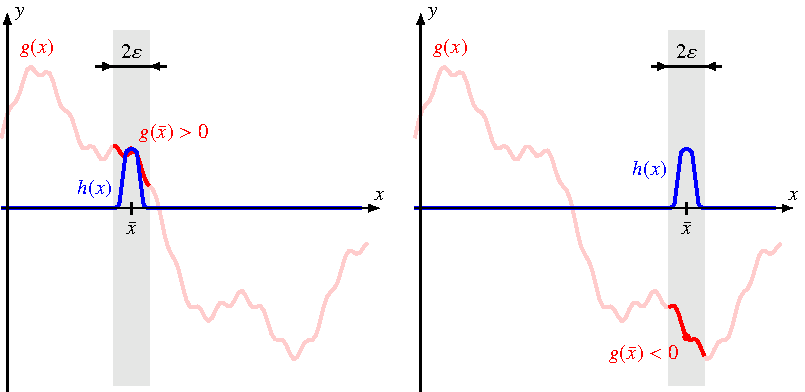
\includegraphics{chapters/30-interpolation/figures/integral.pdf}
\caption{Wenn das Integral von $g(x) h(x)$ für jede Funktion $h(x)$
verschwinden, dann muss auch $g(x)$ verschwinden.
In einer Umgebung eines Punktes $\bar{x}$, wo $g(\bar{x})\ne 0$ ist,
kann man $h(x)$ derart von $0$ verschieden wählen (blaue Kurve),
dass das Integral nicht verschwindet.
Der Widerspruch zeigt, dass $g(\bar{x})=0$ sein muss.
\label{buch:interpolation:figure:integralprinzip}}
\end{figure}

\begin{lemma}[Integralprinzip]
\label{buch:lemma:integralprinzip}
Sei $g(x)$ eine stetige Funktion auf dem Intervall $[a,b]$.
Ausserdem gilt
\[
\int_a^b g(x)  h(x)\,dx = 0
\]
für jede auf $[a,b]$ definierte stetige Funktion mit $h(a)=h(b)=0$.
Dann ist $g(x)=0$.
\end{lemma}

\begin{proof}[Beweis]
Wir führen die Annahme, dass es einen Punkt $\bar{x}$ gibt mit
$g(\bar{x})\ne 0$, zu einem Widerspruch.
\index{Widerspruch}%

Nehmen wir also an, dass $g(\bar{x})>0$ ist.
Dann ist $g(x)>0$ wegen der Stetigkeit von $g$ auch noch ein einer
$\varepsilon$-Umgebung von $\bar{x}$ von $0$ verschieden.
Wir wählen $h(x)$ als stetige Funktion mit folgenden Eigenschaften
\begin{enumerate}
\item
Die Funktion wird nirgends negativ: $h(x)\ge 0$.
\item
$h(x)$ verschwindet ausserhalb der $\varepsilon$-Umgebung von $\bar{x}$.
\item
$h(\bar{x})=1$.
\end{enumerate}
Eine solche Funktion ist in
Abbildung~\ref{buch:interpolation:figure:integralprinzip} links
blau dargestellt.
Da $g(x)$ in der Umgebung $>0$ ist, folgt
\[
\int_a^b g(x)\,h(x)\,dx
=
\int_{\bar{x}-\varepsilon}^{\bar{x}+\varepsilon}
\underbrace{g(x)}_{\displaystyle>0}\,\underbrace{h(x)}_{\displaystyle\ge 0}\,dx
>
0,
\]
im Widerspruch zu den Voraussetzungen.

Der Fall $g(\bar{x})<0$ wird analog dazu behandelt, wie in
Abbildung~\ref{buch:interpolation:figure:integralprinzip} rechts
dargestellt.
\end{proof}

\subsubsection{Beweis von Satz~\ref{buch:satz:eulerlagrange}}
Wir gehen wie folgt vor: wir zeigen zunächst, dass eine solche Funktion
eine Differentialgleichung erfüllen muss.
Dann beziehen wir uns auf bekannte Sätze der Theorie der gewöhnlichen
Differentialgleichungen, die besagen, dass die Gleichung eine glatte 
Lösung hat.

Sei jetzt also $y(x)$ eine Funktion mit $y(a)=y_a$ und $y(b)=y_b$, die
das Integral $J(y)$ minimiert.
Ändern wir die Funktion ein klein wenig, dann muss der Wert von $J$ zunehmen.
Wir vollziehen die Änderung, indem wir eine Funktion $h(x)$
mit $h(a)=0$ und $h(b)=0$ addieren.
Die Funktionen $y_\varepsilon= y+\varepsilon h$ erfüllen dann alle die
Bedingung $y_\varepsilon(a)=y_a$ und $y_\varepsilon(b)=y_b$, insbesondere
müssen sie alle einen Wert $J(g+\varepsilon h)$ ergeben, der grösser ist
als $J(g)$.
Insbesondere muss die Ableitung von $J(y+\varepsilon h)$ nach $\varepsilon$
an der Stelle $\varepsilon=0$ verschwinden.

Wir berechnen die Ableitung von $J(y+\varepsilon h)$ nach $\varepsilon$:
\begin{align}
0
=
\frac{d}{d\varepsilon} J(y+\varepsilon h)\bigg|_{\varepsilon=0}
&=
\frac{d}{d\varepsilon}
\int_a^b L(x, y(x) + \varepsilon h(x), y'(x)+\varepsilon h'(x))\,dx
\bigg|_{\varepsilon=0}
\notag
\\
&=
\int_a^b
\frac{\partial L}{\partial y}(x, y(x), y'(x)) \, h(x)
+
\frac{\partial L}{\partial y_1} L(x, y(x), y'(x)) \, h'(x)
\,dx
\notag
\\
&=
\int_a^b
\frac{\partial L}{\partial y}(x, y(x), y'(x)) \, h(x)
\,dx
+
\int_a^b
\frac{\partial L}{\partial y_1} L(x, y(x), y'(x)) \, h'(x)
\,dx
\label{buch:variation:zweiintegrale}
\end{align}
Das zweite Integral enthält die Ableitung $h'(x)$, über die wir nicht viel
wissen.
Wir können diese aber durch partielle Integration los werden:
\index{partielle Integration}%
\index{Integration!partiell}%
\begin{align*}
\int_a^b
\frac{\partial L}{\partial y_1} L(x, y(x), y'(x)) \, h'(x)
\,dx
&=
\biggl[\frac{\partial L}{\partial y_1}
L(x,y(x),y'(x))\,h(x)
\biggr]_a^b
-
\int_a^b \frac{d}{dx} \frac{\partial L}{\partial y_1}
L(x,y(x),y'(x))\,h(x) \,dx
\intertext{$h$ war so gewählt, dass die Werte, an den Intervallenden
verschwinden, also $h(a)=h(b)=0$.
Der erste Terme verschwindet daher und es bleibt}
&=
-
\int_a^b \frac{d}{dx} \frac{\partial L}{\partial y_1}
L(x,y(x),y'(x))\,h(x) \,dx.
\end{align*}
Einsetzen in \eqref{buch:variation:zweiintegrale} ergibt die Gleichung
\begin{equation}
0=
-
\int_a^b 
\biggl(
\frac{d}{dx}\frac{\partial L}{\partial y_1} (x,y(x), y'(x))
-
\frac{\partial L}{\partial y} (x,y(x),y'(x))
\biggr)
h(x)
\,dx.
\label{buch:variation:eulerintegralform}
\end{equation}

Gleichung \eqref{buch:variation:eulerintegralform}
muss für jede beliebige Funktion $h(x)$ gelten.
Wir möchten zeigen, dass das nur möglich ist, wenn die grosse Klammer
im Integral verschwindet.
Dies ist aber genau die Situation des Integralprinzips von
Lemma~\ref{buch:lemma:integralprinzip}.
\index{Integralprinzip}%
Es gestattet uns zu schliessen, dass das Integral
\eqref{buch:variation:eulerintegralform} nur dann für alle
möglichen Funktionen $h(x)$ verschwindet, wenn die grosse Klammer
im Integranden verschwindet.
Es gilt daher die Gleichung
\begin{equation}
\frac{d}{dx} \frac{\partial L}{\partial y_1} (x,y(x),y'(x)) 
-
\frac{\partial L}{\partial y}L(x,y(x),y'(x)).
\end{equation}
Damit ist der Beweis von Satz~\ref{buch:satz:eulerlagrange} vollständig.

\begin{beispiel}
\index{Euler-Lagrange-Gleichung}%
Wir wenden die Euler-Lagrange-Gleichung auf die Lagrange-Funktion
\eqref{buch:equation:mechlagrange} an, dabei erhalten wir
\[
\left.
\begin{aligned}
\frac{\partial L}{\partial y}
&=
-V'(y)
\\
\frac{\partial L}{\partial\dot{y}}
&=
m\dot{y}
\end{aligned}
\qquad\right\}
\quad\Rightarrow\quad
\frac{d}{dt} \frac{\partial L}{\partial \dot{y}} - \frac{\partial L}{\partial y}
=
\frac{d}{dt} 
m\dot{y} +V'(y)=0
\quad\Rightarrow\quad
m\ddot{y} = -V'(y).
\]
Dies ist das 2.~Newtonsche Gesetz.
\index{2. Newtonsches Gesetz}%
\index{Newtonsches Gesetz, zweites}%
\end{beispiel}

%
% Lösung des Optimierungsproblems
%
\subsection{Lösung des Optimierungsproblems
\label{buch:subsection:splineinterpolant}}
Leider lässt sich der Satz~\ref{buch:variation:eulerlagrange}
nicht direkt auf das Interpolationsproblem anwenden, weil im
Ausdruck $J(g)$ die zweite Ableitung von $g$ vorkommt.
Wir führen daher die Rechnung, die auf die Euler-Lagrange-Differentialgleichung
geführt hat, nochmals in diesem Spezialfall durch.
Wieder sei $h$ eine Funktion, die in jeder Stützstelle verschwindet.
Die Minimalitätsbedingung ist dann
\begin{align}
0
&=
\frac{d}{d\varepsilon}
\int_{x_i}^{x_{i+1}} (g''(x) + \varepsilon h''(x))^2 \,dx\bigg|_{\varepsilon=0}
\notag
\\
&=\int_{x_i}^{x_{i+1}} 2g''(x)h''(x) + 2\varepsilon h''(x)^2\,dx\bigg|_{\varepsilon=0}
\\
\notag
&=
\int_{x_i}^{x_{i+1}} 2g''(x) h''(x)\,dx.
\intertext{Wie bei der Euler-Lagrange-Gleichung können wir durch partielles
Integrieren die zweite Ableitung der Funktion $h$ los werden:}
0
&=
\biggl[ g''(x) h'(x) \biggr]_{x_i}^{x_{i+1}}
-
\int_{x_i}^{x_{i+1}} g'''(x) h'(x) \,dx
\notag
\\
&=
\biggl[ g''(x) h'(x) \biggr]_{x_i}^{x_{i+1}}
-
\biggl[ g'''(x) h(x) \biggr]_{x_i}^{x_{i+1}}
+
\int_{x_i}^{x_{i+1}} g^{(4)}(x) h(x)\,dx.
\label{buch:equation:splines:integiert}
\end{align}
Auf Grund der Definition von $h$ verschwindet der mittlere Term.

%
% Bedingungen im Inneren der Teilintervalle
%
\subsubsection{Bedingungen im Inneren der Teilintervalle}
Jetzt nutzen wir wieder die freie Wahlmöglichkeit der Funktion $h$
aus.
Wir können die Funktion so wählen, dass
$h(x_i)=h(x_{i+1})=h'(x_i)=h'(x_{i+1})=0$ ist, dann 
verschwinden die ersten beiden Terme.
Das Integral verschwindet nur dann immer, wenn der Integrand verschwindet,
wenn also im Inneren jedes Teilintervalls $[x_i,x_{i+1}]$
gilt, dass
$g^{(4)}(x)=0$.
Es folgt, dass in jedem Teilintervall die Funktion $g$ ein kubisches Polynom 
sein muss.

%
% Bedingungen an den Stützstellen
%
\subsubsection{Bedingungen an den Stützstellen}
Aus dem verbleibenden ersten Term von
Gleichung~\eqref{buch:equation:splines:integiert}
lässt sich noch mehr über die zweiten Ableitungen der Funktion $g$
schliessen.
Die Summe dieser Terme muss ja ebenfalls $0$ ergeben, also
\begin{align*}
0
&=
\sum_{i=0}^{n-1} 
\biggl[ g''(x) h'(x) \biggr]_{x_i}^{x_{i+1}}
=
\sum_{i=0}^{n-1}
\bigl( g''(x_{i+1}-) h'(x_{i+1}) - g''(x_i+) h'(x_i) \bigr)
\\
&=
-g''(x_0+)h'(x_0)
+
\sum_{i=1}^{n-1} h'(x_i) \bigl(g''(x_i-) - g''(x_i+)\bigr)
+
g''(x_n-)h'(x_n).
\end{align*}
Indem man für $h$ eine Funktion wählt, die an allen Stützstellen verschwindet
und in genau einer Stützstelle Ableitung $1$ hat, was mit einem
Hermite-Interpolationspolynom sicher möglich ist, schliesst man
\begin{equation}
g''(x_i-)=g''(x_i+)\quad\forall 1\le i< n.
\label{buch:equation:splineinner}
\end{equation}
Die Funktion ist also zweimal stetig differenzierbar.
Schliesslich müssen auch die Terme an den Enden der Summe verschwinden.
Eine Funktion $h$, die in allen Stützstellen zusammen mit der ersten
Ableitung in den inneren Stützstellen verschwindet und deren
erste Ableitung in genau einem der Endpunkte $1$ ist zeigt,
dass ausserdem
\begin{equation}
g''(x_0+) = g''(x_n-) = 0
\label{buch:equation:splinerand}
\end{equation}
sein muss.

%
% Ein Gleichungssystem für die Steigungen
%
\subsubsection{Ein Gleichungssystem für die Steigungen}
Zur Lösung des eingangs gestellten Interpolationsproblems ist jetzt
also für jedes Teilintervall $[x_i,x_{i+1}]$ ein kubisches Polynom $g_i(x)$
zu finden, mit folgenden Eigenschaften:
\begin{align*}
g_i(x_i)     &=f_i       &g_i(x_{i+1})  &=f_{i+1}   &0&\le i\le n &&\text{$2n+2$ Bedingungen}
\\
g_{i-1}'(x_i)&=g_i'(x_i) &g_{i-1}''(x_i)&=g_i''(x_i)&1&\le i< n &&\text{$2n$ Bedingungen}
\\
g_0''(x_0)   &=0         &g_n''(x_n)    &= 0        & &         &&\text{$2$ Bedingungen}
\end{align*}
Dies sind $4n+4$ lineare Bedingungen für $n+1$ Polynome, die je $4$
Koeffizienten haben.
Es sollte sich also ein lineares Gleichungssystem finden lassen, welches
diese Koeffizienten findet.

Aus Abschnitt~\ref{buch:section:hermite} ist bekannt, dass die kubischen
Polynome $g_i(x)$ durch die bereits bekannten Funktionswerte $f_i$
und die noch zu findenen Steigungen in den Stützstellen bestimmt sind.
Wir schreiben daher $s_i = g_i'(x_i)$ für die Steigungen und machen es
uns zum Ziel, ein Gleichungssystem für die $s_i$ zu finden.

In Abschnitt~\ref{buch:subsection:hermite:zweistuetzstellen}
haben wir Hermite-Interopationspolynome für zwei Stützstellen
zusammengestellt.
Wir haben dort die Polynome $H_i$ und $H_i^1$ konstruiert, aus
denen sich mit der Substition $x\to (x-x_0)/m$ die
Hermite-Interpolationspolynome für das Intervall $[x_0,x_0+m]$ 
bilden liess.
Wir bezeichnen die Länge des Intervalls $[x_i,x_{i+}]$
mit $m_i=x_{i+}-x_i$.

Die gesuchte Funktion im Intervall ist daher
\begin{equation}
g_i(x) = f_i H_0((x-x_i)/m_i) + f_{i+1} H_1((x-x_i)/m_i)
+
s_i m_i H_0^1((x-x_i)/m_i) + s_{i+1} m_i H_1^1((x-x_i)/m_i).
\label{buch:equation:spline:loesung}
\end{equation}
Diese Funktion hat die richtigen Funktionswerte und Ableitungen
an den Intervallenden.

Die Steigungen $s_i$ in \eqref{buch:equation:spline:loesung}
ist noch nicht bekannt, aber die Bedingung an die zweiten Ableitungen
wurde noch nicht ausgenutzt.
Die zweiten Ableitungen erfüllen
\begin{align*}
i&=0
&
0
&=
g_0''(x_0)
=
-\frac{6f_0}{m_0^2} + \frac{6f_1}{m_0^2} -\frac{4{\color{red}s_0}}{m_0} + \frac{2{\color{red}s_1}}{m_0}
\\
i&=1
&
&\phantom{\mathstrut=\mathstrut}
g_0''(x_1)
=
\phantom{-}
\frac{6f_0}{m_0^2} -\frac{6f_1}{m_0^2} +\frac{2{\color{red}s_0}}{m_0} -\frac{4{\color{red}s_1}}{m_0}
\\
&
&
&=
g_1''(x_1)
=
-\frac{6f_1}{m_1^2}+\frac{6f_2}{m_1^2} - \frac{4{\color{red}s_1}}{m_1}+\frac{2{\color{red}s_2}}{m_1}
\\
i&=2
&
&\phantom{\mathstrut=\mathstrut}
g_1''(x_2)
=
\phantom{-}
\frac{6f_1}{m_1^2} -\frac{6f_2}{m_1^2} +\frac{2{\color{red}s_1}}{m_1} -\frac{4{\color{red}s_2}}{m_1}
\\
&
&
&=
g_2''(x_2)
=
-\frac{6f_2}{m_2^2}+\frac{6f_3}{m_2^2} - \frac{4{\color{red}s_2}}{m_2}+\frac{2{\color{red}s_3}}{m_2}
\\
&\qquad\vdots
&&
\\
i&=n
&
0&=
g_n''(x_n)
=
\phantom{-}
\frac{6f_{n-1}}{m_n^2}-\frac{6f_n}{m_n^2} +\frac{2{\color{red}s_{n-1}}}{m_n}-\frac{4{\color{red}s_n}}{m_n}.
\end{align*}
In allen Gleichungen kommt der Faktor $2$ vor, den wir herausdividieren 
können.
Schaffen wir die Terme in $f_i$ auf die rechte Seite und sammeln die
Terme mit ${\color{red}s_i}$ auf der linken Seite, erhalten wir das
Gleichungssystem
\begin{equation}
\begin{linsys}{6}
\displaystyle\frac{2}{m_0} {\color{red}s_0}
	&+&\displaystyle \frac{1}{m_0}{\color{red}s_1}
		& &
			& &
				& &
				& &
					&=&\displaystyle3\frac{f_1-f_0}{m_0^2}
\\
\displaystyle \frac{1}{m_0} {\color{red}s_0}
	&+&\displaystyle \biggl(\frac{2}{m_0}+\frac{2}{m_1}\biggr){\color{red}s_1}
		&+& \displaystyle \frac{1}{m_1}{\color{red}s_2}
			& &
				& &
				& &
					&=&\displaystyle3\frac{f_2-f_1}{m_1^2}
\\
	& &\displaystyle\frac{1}{m_1} {\color{red}s_1}
		&+&\displaystyle\biggl(\frac{2}{m_1}+\frac{2}{m_2}\biggr) {\color{red}s_2}
			&+& \displaystyle\frac{1}{m_2} {\color{red}s_3}
				& &
				& &
					&=&\displaystyle3\frac{f_3-f_2}{m_2^2}
\\
	& &
		& &
			& &
				&\ddots&
				&\ddots&
					& &\vdots\hspace*{10pt}
\\
	& &
		& &
			& &
			& &\displaystyle \frac{1}{m_{n-2}}{\color{red}s_{n-1}}
				&+&\displaystyle \frac{2}{m_{n-1}}{\color{red}s_n}
					&=&\displaystyle3\frac{f_n-f_{n-1}}{m_{n-1}^2}
\end{linsys}
\end{equation}
Die Koeffizientenmatrix und die rechte Seite dieses Gleichungssytems sind
\[
A
=
\begin{pmatrix}
\displaystyle\frac{2}{m_0}
	&\displaystyle\frac{1}{m_0}
		&
			&
				&
					&
\\[8pt]
\displaystyle\frac{1}{m_0}
	&\displaystyle\frac{2}{m_0}+\frac{2}{m_1}
		&\displaystyle\frac{2}{m_1}
			&
				&
					&
\\[8pt]
	&\displaystyle\frac{1}{m_1}
		&\displaystyle\frac{2}{m_1}+\frac{2}{m_2}
			&\displaystyle\frac{1}{m_2}
				&
					&
\\[8pt]
	&
		&\displaystyle\frac{1}{m_2}
			&\ddots
				&\ddots
					&
\\[8pt]
	&
		&
			&\ddots
				&\ddots
					&\displaystyle\frac{1}{m_{n-2}}
\\[8pt]
	&
		&
			&
				&\displaystyle\frac{1}{m_{n-2}}
					&\displaystyle\frac{2}{m_{n-1}}
\end{pmatrix}
\qquad\text{und}\qquad
b
=
\begin{pmatrix}
\displaystyle3\frac{f_1-f_0}{m_0^2} \\[8pt]
\displaystyle3\frac{f_2-f_1}{m_1^2} \\[8pt]
\displaystyle3\frac{f_3-f_2}{m_2^2} \\[8pt]
\vdots \\[8pt]
\displaystyle3\frac{f_{n-1}-f_{n-2}}{m_{n-2}^2} \\[8pt]
\displaystyle3\frac{f_n-f_{n-1}}{m_{n-1}^2} 
\end{pmatrix}.
\]
Die Gleichungen werden besonders einfach, wenn alle Abstände gleich sind,
zum Beispiel $m=m_0=\dots =m_{n-1}$.
Dann kann man die Gleichungen mit $m$ multiplizieren und bekommt für die
Koeffizientenmatrix und die rechte Seite
\[
A
=
\begin{pmatrix}
2&1& &      &      & \\
1&2&1&      &      & \\
 &1&2&1     &      & \\
 & &1&\ddots&\ddots& \\
 & & &\ddots&\ddots&1\\
 & & &      &     1&2
\end{pmatrix}
\qquad\text{und}\qquad
b
=
\frac{3}{m}
\begin{pmatrix}
f_1-f_0\\
f_2-f_1\\
f_3-f_2\\
\vdots\\
f_{n-1}-f_{n-2}\\
f_n-f_{n-1}
\end{pmatrix}
\]
Nach Lösung dieses Gleichungssystems kann man in jedem Teilintervall
$[x_i,x_{i+1}]$ mit Hilfe des kubischen Hermite-Interpolationspolynoms
eine Spline-Interpolationsfunktion konstruieren.
\index{Hermite-Interpolationspolynom}%
\index{Spline-Interpolationsfunktion}%

%
% bezier.tex
%
% (c) 2020 Prof Dr Andreas Müller, Hochschule Rapperswil
%

\subsection{Bézier-Kurven und Splines in der Ebene
\label{buch:subsection:bezier}}
Spline-Interpolation kann auch verwendet werden um Kurven in der Ebene
oder im Raum zu approximieren.
In der Computergraphik ist dabei besonders wichtig, dass sich Kurvenpunkte
mit einfachen Operationen aus einer kleinen Zahl von Parametern berechnen
lassen, damit sie zum Beispiel von einem Graphikprozessor berechnet
werden können.
Dieser Abschnitt soll daher den Zusammenhang zwischen Bézier-Kurven und
Splines aufzeigen.


\subsubsection{Kurven in der Ebene}
Eine Kurve in der Ebene ist eine Abbildung
\[
\gamma \colon \mathbb R \to \mathbb R^2 : t \mapsto \gamma(t) = (x(t),y(t)),
\]
genannt die Parameterdarstellung der Kurve.
Man kann sich den Parameter $t$ als die Zeit vorstellen und die Funktionen
$x(t)$ bzw.~$y(t)$ als die Koordinaten eines sich auf der Kurve bewegenden
Punktes zur Zeit $t$.
Der Tangentialvektor
\[
\dot{\gamma}(t)
=
\frac{d\gamma(t)}{dt}
=
\begin{pmatrix}
\dot{x}(t)\\\dot{y}(t)
\end{pmatrix}
\]
kann entsprechend auch als der Geschwindigkeitsvektor zur Zeit $t$ 
intepretiert werden.

\begin{beispiel}
Ein Kreis in der Ebene kann beschreiben weren mit der Parameterisierung
\[
\gamma(t) = (\cos t, \sin t)
\qquad
\text{mit Geschwindigkeitsvektor}
\qquad
\dot{\gamma}(t)
=
\begin{pmatrix}
-\sin t\\\cos t
\end{pmatrix}.
\]
Der Betrag der Geschwindigkeit ist $|\dot{\gamma}(t)|^2=\sin^2t+\cos^2t=1$,
also konstant.
\end{beispiel}

\begin{beispiel}
Jeder Graph einer Funktion $f(x)$ kann als Kurve mit der Parameterisierung
\[
\gamma \colon \mathbb R\to\mathbb R^2 : t \mapsto (t, f(t))
\]
aufgefasst werden.
Der Tangentialvektor ist
\[
\dot{\gamma}(t)
=
\begin{pmatrix}
1\\f'(t)
\end{pmatrix}.
\]
Insbesondere ist die Geschwindigkeit $|\dot{\gamma}(t)|^2=1+f'(x)^2|>1$
im Allgemeinen nicht konstant.
\end{beispiel}

Das Beispiel zeigt, dass Graphen von Funktionen zwar als Kurven aufgefasst
werden können, als Bahnbeschreibung zum Beispiel für einen Roboter taugen
sie dagegen kaum.
Andererseits haben die Spline-Interpolationsfunktionen die schöne
Eigenschaft, dass die mittlere zweite Ableitung minimiert wird.
Sie sind daher ``die am wenigsten gekrümmten'' Kurven, die durch die
Stützstellen gehen. 
Eine solche Minimaleigenschaft für die Bahnkurve eines Roboters könnte eine
Bahn beschreiben, die sich mit maximaler Geschwindigkeit durchfahren lässt.
Die Zentripetalkraft, die die Räder in den Kurven aufbringen müssen,
kann nicht grösser sein als die Haftreibung.
Je grösser die Bahnkrümmung, desto grösser auch die Zentripetalkraft und
desto langsamer muss der Roboter durch die Kurve fahren, um nicht ins
Rutschen zu geraten.

Wir betrachten also eine Kurve, die durch die vorgegebene Punkte
\[
P_0 = (x_0, y_0),\;
P_1 = (x_1, y_1), \;
P_2 = (x_2, y_2),
\dots,
P_n=(x_n, y_n)
\]
gehen soll.
Wir fordern, dass der Punkt $P_i$ zum Zeitpunkt $t_i$ durchlaufen wird.
Wir entfernen uns hier etwas von der Anwendung einer Robotersteuerung,
da würde man nur die Punkte vorgeben und dann eine Bahn suchen, mit der
sich die Zeitpunkte $t_i$ so wählen lassen, dass die Gesamtzeit minimal
wird.
Die Funktionen $x(t)$ und $y(t)$ erfüllen jetzt also
\[
x(t_i) = x_i
\qquad\text{und}\qquad
y(t_i) = y_i.
\]
Das Problem, eine ebene Kurve durch die Punkte $P_i$ zu parametrisieren
ist jetzt also zerlegt worden in zwei unabhängige Interolationsprobleme
für die Funktionen $x(t)$ und $y(t)$.

Jedes in diesem Kapitel besprochene Interpolationsverfahren kann dafür
eine mögliche Lösung liefern, wobei sich die Spline-Interpolation wegen
der genannten Minimaleigenschaft besonders aufdrängt.
Dabei müssen zuerst die Steigungen und den Knotenstellen $t_i$ ermittelt
werden,
aus denen sich dann mittels Hérmite-Interpolation die Kurvenstücke
zwischen den Punkten $P_i$ als kubische Kurven berechnen lassen.
Die Steigungen in den Knotenstellen $t_i$ sind die Ableitungen
$\dot{x}(t_i)$ und $\dot{y}(t_i)$, d.~h.~es wir müssen zwischen
$P_i$ und $P_{i+1}$ eine kubische Kurve in der Ebene berechnen, die
Tangentialvektor $(\dot{x}(t_i),\dot{y}(t_i))^t$
bzw.~$(\dot{x}(t_{i+1}),\dot{y}(t_{i+1}))^t$ haben.
Eine besonders elegante Lösung für dieses Problem sind die Bézier-Kurven.

\subsubsection{Bézier-Kurven}
\begin{figure}
\centering
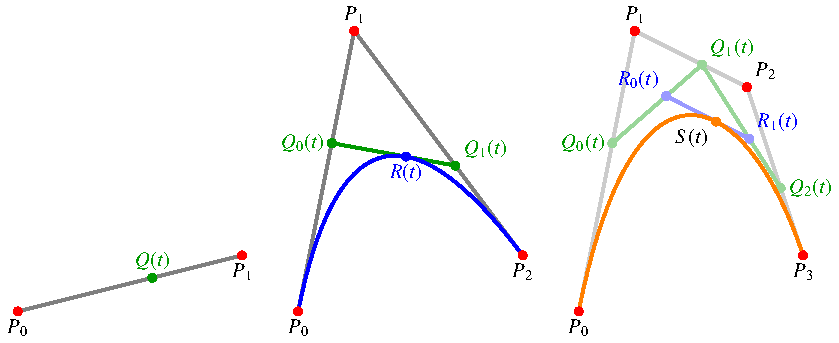
\includegraphics{chapters/30-interpolation/figures/bezier.pdf}
\caption{Bézier-Kurven bis zur Ordnung 3
\label{buch:interpolation:figure:bezier}}
\end{figure}
Die einfachste Verbindung zwischen zwei Punkten $P_0$ und $P_1$ mit
Ortsvektoren $p_0$ und $p_1$ ist eine Strecke, die man mit
\[
\gamma(t) = (1-t)p_0 + tp_1
\]
parametrisieren kann.
Der Tangentialvektor ist bereits bestimmt, er ist
\[
\dot{\gamma}(t) = -p_0 + p_1 = p_1-p_0.
\]
Die zwei Punkte legen den Tangentialvektor bereits fest, man kann
ihn nicht mehr frei wählen.

Kann man eine einfach zu berechnende Kurve finden, die den Punkt $P_0$
mit einem vorgegebenen Geschwindigkeitsvektor verlässt?
Paul de Casteljau hat vorgeschlagen, drei Punkte $P_0$, $P_1$ und $P_2$
zu verwenden und zunächst wie vorhin die Strecken 
\begin{align*}
q_0(t) &= (1-t) p_0 + t p_1 \\
q_1(t) &= (1-t) p_1 + t p_2 
\end{align*}
zu bilden.
Zur Zeit $t=0$ verlässt das erste Segment den Punkt $P_0$ mit der
Geschwindigkeit $p_1-p_0$.
Zur Zeit $t=1$ kommt das zweite Segment im Punkt $P_2$ an mit der
Geschwindigkeit $p_2-p_1$.
Man muss also zwischen $t=0$ und $t=1$ ``vom ersten Segment auf das zweite
wechseln''.
Dazu verbindet man die Punkte $q_0(t)$ und $q_1(t)$ mit einer Strecke und
wähle den Streckenparameter wieder als $t$.
Man erhält so eine Kurve
\begin{align*}
r(t)
&=
(1-t) q_0(t) + t q_1(t)
\\
&=
(1-t) \bigl( (1-t)p_0 + tp_1\bigr)
+
t \bigl( (1-t)p_1 + tp_2\bigr)
\\
&=
(1-t)^2 p_0 + 2t(1-t) p_1 + t^2 p_2.
\end{align*}
Der Geschwindigkeitsvektor zu den Zeiten $t=0$ und $t=1$ ist
\begin{align*}
\dot{r}(t)
&=
-2(1-t)p_0 + (2(1-t)-2t) p_1 + 2tp_2
\\
&=\begin{cases}
-2p_0+2p_1=2(p_1-p_0)&\qquad t=0
\\
-2p_1+2p_2=2(p_2-p_1)&\qquad t=1
\end{cases}
\end{align*}
Die gefundene Kurve verlässt also den Punkt $P_0$ genau in Richtung
auf $P_1$ und kommt im Punkt $P_2$ aus der Richtung von $P_1$ an.
Wir haben also eine quadratische Kurve gefunden, die einen Teil 
der Forderungen erfüllt.

Man nennt diese Kurve eine quadratische {\em Bézier-Kurve} mit
\index{Bézier-Kurve}
{\em Kontrollpunkten} $P_0$, $P_1$ und $P_2$.
\index{Kontrollpunkte}
Der Punkt $P_1$ kontrolliert die Start- und Ankunftsrichtung.

Die beiden Richtungen in Anfangs- und Endpunkten müssen unabhängig
voneinander vorgegeben werden können, wir versuchen daher, die
gleiche Konstruktion mit vier Kontrollpunkten durchzuführen.
Gegeben seien jetzt also die Punkte $P_0,\dots,P_3$.
Dann können wir drei Strecken
\begin{align*}
q_0(t) &= (1-t) p_0 + t p_1 \\
q_1(t) &= (1-t) p_1 + t p_2 \\
q_2(t) &= (1-t) p_2 + t p_3 
\end{align*}
konstruieren.
Die erste hat die ``richtige'' Startrichtung, die letzte die ``richtige''
Ankunfsrichtung.
Kombinieren wir $q_0(t)$ und $q_1(t)$, erhalten wir eine quadratische
Kurve, die vom Punkt $P_0$ mit der richtigen Geschwindigkeit weggeht,
die Kombination von $q_1(t)$ mit $q_2(t)$ liefert eine quadratische
Bézier-Kurve, welche im Punkt $P_3$ mit der richtigen Geschwindigkeit
ankommt.
Wir können also erneut kombinieren:
\begin{equation}
\left.
\begin{aligned}
r_0(t) &= (1-t)q_0(t) + t q_1(t) \\
       &= (1-t)^2 p_0 + 2t(1-t) p_1 + t^2 p_2
\\
r_1(t) &= (1-t)q_1(t) + t q_2(t) \\
       &= (1-t)^2 p_1 + 2t(1-t) p_2 + t^2 p_3
\end{aligned}
\quad
\right\}
\quad\Rightarrow\quad
s(t) = (1-t) r_0(t) + t r_1(t)
\end{equation}
Wir berechnen 
\begin{equation*}
\begin{linsys}{5}
s(t) &=& (1-t) \bigl( (1-t)^2 p_0 &+& 2t(1-t)         p_1 &+& t^2     p_2 &\bigr) & \phantom{\bigr)}\\
     & &                          & & t\bigl( (1-t)^2 p_1 &+& 2t(1-t) p_2 &+& t^2p_3\bigr) \\
     &=& (1-t)^3 p_0 &+& 3t(1-t)^2 p_1 &+& 3t^2(1-t) p_2 &+& t^3 p_3\rlap{.}\phantom{\bigr)}
\end{linsys}
\end{equation*}
Der Tagententialvektor an den Stellen $t=0$ und $t=1$ ist
\begin{align*}
\dot{s}(t)
&=
-3(1-t)^2p_0 + (3(1-t)^2-6t(1-t))p_1 + (6t(1-t)-3t^2)p_2 + 3t^2p_3
\\
\Rightarrow\qquad
\dot{s}(0) &= -3p_0+3p_1 = 3(p_1-p_0)
\\
\dot{s}(1) &= -3p_2 + 3p_3 = 3(p_3-p_2),
\end{align*}
die Kurve verlässt also wie erwartet den Punkt $P_0$ genau in Richtung 
auf $P_1$ und kommt genau aus der Richtung von $P_2$ in $P_3$ an.

Man kann auch die Spline-Funktionen wieder aus der zweidimensionalen
Kurve $s(t)$ rekonstruieren.
Gegeben sind dafür zwei Werte $y_0$ und $y_1$ und die Steigungen $m_0$ und
$m_1$ in den Punkten $x=0$ und $x=1$.
Der Graph des kubischen Polynoms $p(x)$ mit $p(0)=y_0$, $p(1)=y_1$,
$p'(0)=m_0$ und $p'(1)=m_1$ soll jetzt als Bézier-Kurve geschrieben werden.
Dazu müssen die Kontrollpunkte gefunden werden.
Es ist klar, dass $P_0=(0,y_0)$ und $P_3=(1,y_1)$.
Für die inneren Kontrollpunkte muss ein geeigneter $x$-Wert gewählt werden,
also
\[
P_1=
(x_1,y_0+x_1m_0)
\qquad
\text{und}
\qquad
P_2
=
(x_2,y_1-(1-x_2)m_1)
\]
Wählt man $x_1=\frac13$ und $x_2=\frac23$, dann wird
\begin{align*}
x(t)
&=
(1-t)^3\cdot 0 + 3t(1-t)^2\cdot \frac13 + 3t^2(1-t)\cdot \frac23 + t^3\cdot 1
\\
&=
t-2t^2+t^3 + 2t^2 -2t^3 + t^3 = t.
\end{align*}
Mit dieser Wahl ist also $x=t$, so dass das gesuchte Polynom $p(x)=y(x)$ wird:
\begin{align*}
p(x)
=
y(x)
&=
(1-x)^3 y_0
+
3x(1-x)^2\biggl(y_0+\frac13m_0\biggr)
+
3x^2(1-x) \biggl(y_1-\frac13m_1\biggr)
+
x^3 y_1
\\
&=
\bigl((1-x)^3+3x(1-x)^2\bigr)
y_0
+
x(1-x)^2 m_0
-
x^2(1-x) m_1
+
\bigl(3x^2(1-x)+x^3\bigr)
y_1
\\
&=
(1+2x)(1-x)^2 y_0
+
x(1-x)^2 m_0
+
x^2(x-1) m_1
+
x^2(3-2x) y_1.
\end{align*}
Die Koeffizienten von $y_0$, $y_1$, $m_0$ und $m_1$ sind die Polynome
\begin{equation}
\begin{aligned}
y_0:&&
H_0(x)
&=
2x^3-3x^2+1
&\quad&
&m_0:&&
H_0^1(x)
&=
x-2x^2+x^3
\\
y_1:&&
H_1(x)
&=
3x^2-2x^3
&\quad&
&m_1:&&
H_1^1(x)
&=
x^3-x^2
\end{aligned}
\label{buch:bezier:eqn:H}
\end{equation}
Die Polynome \eqref{buch:bezier:eqn:H} stimmen mit den Polynomen überein,
die in \eqref{buch:equation:hermite:h} gefunden worden sind.






\section*{Übungsaufgaben}
\aufgabetoplevel{chapters/30-interpolation/uebungsaufgaben}
\begin{uebungsaufgaben}
\uebungsaufgabe{3001}
\uebungsaufgabe{3002}
\uebungsaufgabe{3003}
\end{uebungsaufgaben}
